Απαραίτητη φάση της διαδικασίας εξόρυξης δεδομένων είναι η συλλογή και η προετοιμασία των δεδομένων. Η φάση κατανόησης των δεδομένων περιλαμβάνει τη συλλογή και εξερεύνησή τους. Ρίχνοντας μια πιο προσεκτική ματιά στα δεδομένα, καθίσταται εφικτός ο καθορισμός του πόσο καλά μπορούμε να αντιμετωπίσουμε το πρόβλημα. Η προσεκτική προετοιμασία δεδομένων μπορεί να βελτιώσει δραστικά τις πληροφορίες που μπορούν να εξαχθούν από την εξόρυξη δεδομένων\cite{miningOracle}.
\section{Περιγραφή δεδομένων}
Τα δεδομένα υπό εξερεύνηση αποτελούνται από καταναλώσεις έξυπνων μετρητών για σχεδόν 5.000 οικιακά νοικοκυριά και 600 επιχειρήσεις. Πιο συγκεκριμένα προέρχονται από την \en{Commision for Energy Regulation (CER)}, η οποία αποτελεί την ανεξάρτητη αρχή για ενέργεια και νερό της Ιρλανδίας \cite{cer}. Οι ενδιαφερόμενοι πελάτες παρείχαν εθελοντικά τα δεδομένα των καταναλώσεων και ερωτηματολόγια για τις καταναλωτικές τους συνήθειες και τις υποδομές τους πράγμα που δίνει τη δυνατότητα να αναλυθούν διεξοδικά τα δεδομένα. Τα αντιπροσωπευτικά αυτά δείγματα συλλέχθηκαν ανώνυμα σε χρονικό παράθυρο σχεδόν 2 ετών, από το (2009-2011) και με συχνότητα λήψης 30 λεπτά για αυτό το διάστημα. Οι πληροφορίες των έξυπνων μετρητών είναι αποθηκευμένες σε έξι διαφορετικά αρχεία κειμένου (\en{.txt}), που καθένα έχει 24 εκατομμύρια καταχωρήσεις που αντιστοιχούν σε διάφορες μετρήσεις ενέργειας. Ο Πίνακας \ref{tab:rawdata} αντιπροσωπεύει ένα μικρό δείγμα των αρχείων κειμένου, το οποίο αποτελείται από 3 στήλες. Η πρώτη στήλη αναπαριστά το \en{ID} του έξυπνου μετρητή που είναι ξεχωριστό για κάθε νοικοκυριό. Η δεύτερη στήλη δείχνει την ημερομηνία και την ώρα που σχετίζεται με τη συγκεκριμένη μέτρηση, ενώ η τρίτη στήλη αποτελεί την αντίστοιχη μέτρηση ενέργειας που καταναλώθηκε σε κιλοβατώρες (\en{kWh})\cite{rawdataNN}.
\begin{table}[ht!]
\centering
\begin{tabular}{ |c|c|c|  }
 \hline
 \en{ID} Μετρητή & Κωδικοποιημένη ημερομηνία/ώρα & Κατανάλωση ενέργειας \en{kWh} \\
 \hline
 1392 & 19503 & 0.140\\
  \hline
 1392 & 19504 & 0.138\\
  \hline
 ... & ... & ...\\
  \hline
 1187 & 22028 & 1.367\\
  \hline
 1187 & 22029 & 1.425\\
 \hline
 1392 & 19940 & 0.234\\
 \hline
\end{tabular}
\caption{Στιγμιότυπα αρχείου δεδομένων}
\label{tab:rawdata}
\end{table}
\subsection{Επισκόπηση χρονοσειρών}
Έχοντας διευκρινίσει, λοιπόν την προέλευση και τη δομή των δεδομένων αξίζει να γίνει μια αναλυτική επισκόπηση τους. Επειδή, καθίσταται αδιανόητη η μελέτη 4.500 ετήσιων καταναλώσεων, επιλέγονται ομάδες που να αντιπροσωπεύουν τον πληθυσμό.  Για να μπορέσει να γίνει αυτό δημιουργήθηκαν 6 συστάδες (ομάδες) που να εκφράζουν είτε τη μορφή της καμπύλης είτε το ύψος της ημερήσιας κατανάλωσης. Με αυτό τον τρόπο ομαδοποιούνται τα δεδομένα και διευκολύνεται η διαδικασία παρατήρησης των χαρακτηριστικών 6 διαφορετικών ομάδων βάση 2 διαφορετικών κριτηρίων. Επιλέχθηκαν 6 συστάδες, καθώς έτσι επιτυγχάνεται ομοιομορφία στο πλήθος των μελών. Άμεσο αποτέλεσμα είναι οι συστάδες να αντιπροσωπεύουν κάποιο μετρήσιμο πλήθος μέλων. Στον Πίνακα \ref{tab:2waycluster} φαίνονται τα αποτελέσματα με τα μέλη κάθε συστάδας:

\begin{table}[ht!]
\centering
 \begin{subfigure}[b]{0.3\textwidth}
\begin{tabular}{ |c|c|  } 
 \hline
 Συστάδα & Μέλη \\
 \hline
 1   &   1083  \\
2   &   351  \\
3   &  544  \\
 4   &   1078 \\
 5   &   420  \\
   6 &1024 \\
   \hline
\end{tabular}
\caption{Συσταδοποίηση βάση των μορφών των χρονοσειρών}
\label{tab:formcluster}
\end{subfigure}
%\end{table}
\quad
%\begin{table}[ht!]
%\centering
\begin{subfigure}[b]{0.4\textwidth}
\begin{tabular}{ |c|c|c|  }
 \hline
 Συστάδα & Μέλη & Μέση κατανάλωση(\en{kWh})\\
 \hline
   1   &   1680  & 26.75\\
  2   &   163  & 77.35\\ 
  3   &   721  &42.67\\ 
  4   &   49  &330.51\\ 
  5   &   1795 &13.36\\ 
  6   &   92  &157.39\\
   \hline
\end{tabular}
\caption{Συσταδοποίηση βάση του ύψους της κατανάλωση} 
\label{tab:conscluster}
\end{subfigure}
\caption{Ομαδοποιήσεις με 2 κριτήρια}
\label{tab:2waycluster}
\end{table}
Παρατηρείται, λοιπόν πως στον Πίνακα \ref{tab:formcluster} η συσταδοποίηση βάση των μορφών των χρονοσειρών έχει 3 πολυμελείς συστάδες που συνοψίζουν τους 3.185 από τους 4.500 που επιλέχθηκαν για τη δοκιμή δημιουργώντας σχετικά ομοιόμορφες συστάδες. Παράλληλα, στον Πίνακα \ref{tab:conscluster} η συσταδοποίηση βάση του ύψους της κατανάλωσης έχει 2 πολυμελείς συστάδες που συνoψίζουν τους 3.475 από τους 4.500 που επιλέχθηκαν και πρόκειται για απλούς οικιακούς πελάτες κρίνοντας από την μέση ημερήσια κατανάλωση κάθε συστάδας. Δεν μπορεί να παραληφθεί σε αυτό το σημείο το γεγονός πως υπάρχουν 2 ολιγομελείς ομάδες που απαριθμούν αθροιστικά 141 μέλη και έχουν πολλαπλάσιες ημερήσιες καταναλώσεις από τους υπόλοιπους.\par
Για περαιτέρω εξερεύνηση των κριτηρίων ομαδοποίησης και των συστάδων δημιουργήθηκαν 2 σχήματα που αποτελούνται από παραδείγματα μελών κάθε συστάδας. Αναλυτικότερα στο Σχήμα \ref{fig:clusterform} και στο Σχήμα \ref{fig:clusterconslevel} φαίνονται τυχαία επιλεγμένες καταναλώσεις για κάθε συστάδα. Έτσι δίνεται η δυνατότητα να αναλύσουμε τη μορφή 6 διαφορετικών ομάδων, αλλά και να παρατηρούμε τον διαχωρισμό των καταναλωτών και τις χρονοσειρές του με γνώμονα την ημερήσιά του κατανάλωση σε διάρκεια ενός έτους.
\begin{figure}[ht!]
\centering
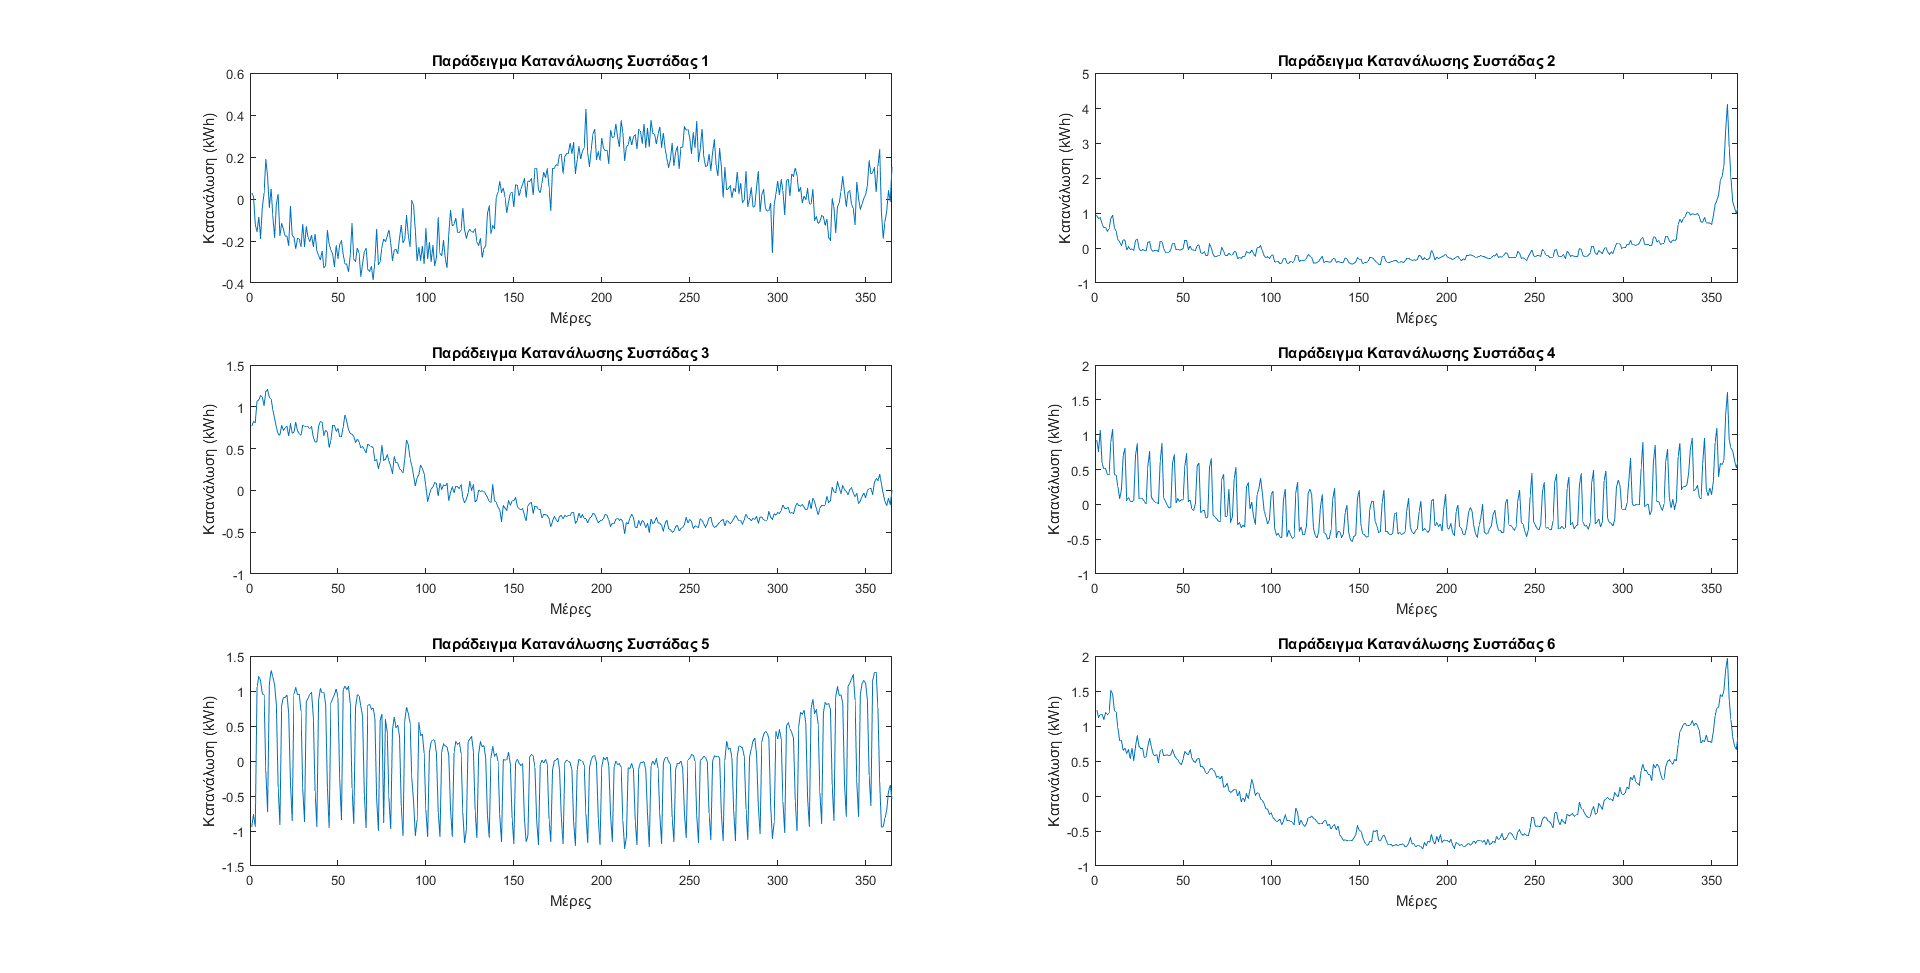
\includegraphics[width=180mm, height=100mm]{../../plots/Consumption_Analysis/gr_cluster_form.png}
\caption{Παραγείματα χρονοσειρών συσταδοποίησης βάση της μορφής των χρονοσειρών}
\label{fig:clusterconslevel}
\end{figure}
Όπως φαίνεται παραπάνω υπάρχουν κάποιες αξιοσημείωτες ομοιότητες και διαφορές μεταξύ των μορφών των καμπυλών.
\begin{itemize}
\item Η συστάδα 1 φαίνεται πως στο ενδιάμεσο του έτους έχει μείωση της κατανάλωσης, ενώ κοντά στο χειμώνα οπού ξεκινά και τελειώνει η χρονοσειρά αύξησή της. 
\item Η συστάδα 2 έχει πολύ έντονες και συνεχείς διακυμάνσεις αλλά κρατά σχεδόν σταθερό μέσο όρο ανά της ημέρες, καθώς η διακύμναση είναι έντονη αλλά γύρω από μια νοητή γραμμή με ελάχιστη κλίση. Παράλληλα, είναι εμφανές πως στους χειμερινούς μήνες έχουμε αισθητή αύξηση της κατανάλωσης.
\item Η συστάδα 3 εμφανίζει μια σχετικά ακανόνιστη, αλλά φθίνουσα εν γένει πορεία. Ειδικότερα υπάρχουν 2 σημαντικές βυθίσεις μία το Καλοκαίρι και μία το Φθινόπωρο. 
\item Η συστάδα 4 θυμίζει σημαντικά λευκό θόρυβο, καθώς δεν παρατηρείται έντονη απόκλιση από την μέση τιμή της καμπύλης, ενώ παράλληλα υπάρχει έντονος βαθμός τυχαιότητας στις διακυμάνσεις με την κατανάλωση να αυξάνεται μόνο τον τελευταίο μήνα του έτους.
\item Η συστάδα 5 σημειώνει μια ύφεση στην κατανάλωση στο τέλος του χειμώνα που επιστρέφει στα κανονικά της επίπεδα μέσα στην άνοιξη. Κατά τα άλλα δεν φαίνεται να έχει κάποια άλλη έντονη κλίση.
\item Η συστάδα 6 έχει εμφανώς αρχικά φθίνουσα τάση, ενώ μετά το καλοκαίρι ξεκινά βίαια και μετά ομαλότερα να αυξάνεται η ημερήσια κατανάλωση.
\end{itemize}
\begin{figure}[ht!]
\centering
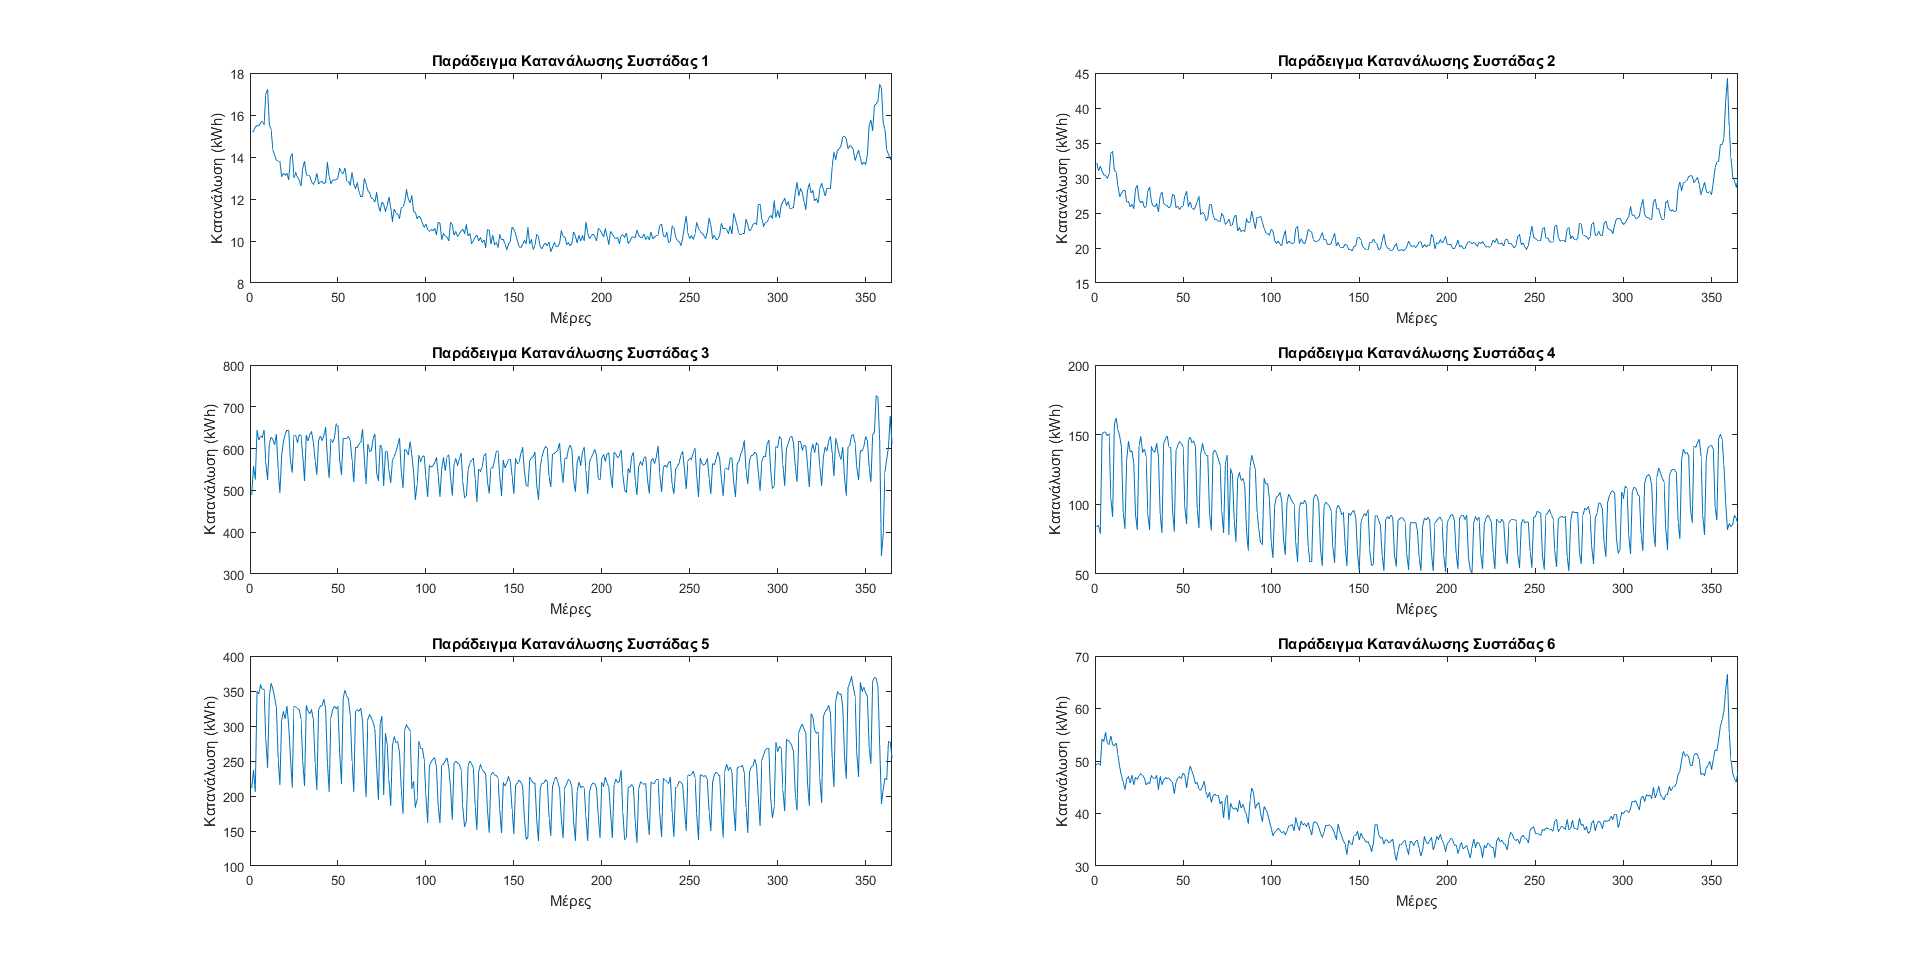
\includegraphics[width=180mm, height=100mm]{../../plots/Consumption_Analysis/gr_cluster_cons_level.png}
\caption{Παραγείματα χρονοσειρών συσταδοποίησης βάση του ύψους της κατανάλωση}
\label{fig:clusterform}
\end{figure}
Στο παραπάνω Σχήμα εμφανίζονται τα παραδείγματα των συστάδων που δημιουργήθηκαν βάση του ύψους των ημερήσιων καταναλώσεων με τις εξής επισημάνσεις:
\begin{itemize}
\item Η συστάδα 1 που αποτελεί τη 2η μεγαλύτερη συστάδα έχει τιμές που κυμαίνονται γενικώς γύρω στις 27 \en{kWh} με 2 κύριες αλλαγές στη μονοτονία.
\item Η συστάδα 2 εμπεριέχει καταναλωτές μικρομεσσαίων επιχειρήσεων με έντονες διακυμάνσεις και σχετικά μεγάλες καταναλώσεις.
\item Η συστάδα 3 δεν έχει κάποιο ιδιαίτερο χαρακτηριστικό, καθώς εμφανίζει εξαιρετικές ομοιότητες με τη συστάδα 1 με μόνη διαφορά την μικρότερη κλίση στις μονοτονίες.
\item Η συστάδα 4 εμφανίζει πολύ ξεχωριστή συμπεριφορά όντας καμπύλη μιας επιχείρησης με μεγάλες ενεργειακές απαιτήσεις που εμφανίζει τη μέγιστή της ζήτηση μετά τους καλοκαιρινούς μήνες. 
\item Η συστάδα 5 περιλαμβάνει ένα μεγάλο μέρος των οικιακών καταναλωτών που έχουν προσγειωμένες τιμές ημερήσιας κατανάλωσης, αλλά και μικρές διακυμάνσεις στη μονοτονία και στις μετρήσεις τους.
\item Η συστάδα 6 περιγράφει καταναλωτές επιχειρήσεων με έντονη διακύμανση της κατανάλωσης ξεκινώντας με έντονη φθίνουσα πορεία και ακολουθώντας με ομαλή αύξουσα πορεία μετά το καλοκαίρι.
\end{itemize}
\subsubsection{Ιστογράμματα Συχνοτήτων}
Για την δημιουργία του ιστογράμματος απαιτείται ένα διάνυσμα δεδομένων που επιλέχθηκε να είναι ο μέσος  όρος και η τυπική απόκλιση των ημερήσιων καταναλώσεων και η ετήσια κατανάλωση πελατών. Ο σκοπός ενός ιστογράμματος είναι να αναπαριστά γραφικά την κατανομή των δεδομένων με εξάρτηση από μια μεταβλητή. Το ιστόγραμμα χρησιμοποιείται ευρέως για να δώσει απάντηση στα παρακάτω ερωτήματα\cite{histogram}:
\begin{enumerate}
\item Τι είδους κατανομή ακολουθεί ο πληθυσμός?
\item Που τοποθετούνται τα δεδομένα στον οριζόντια άξονα?
\item Πόσο αραιά είναι?
\item Υπάρχει εμφανής συμμετρία ή κυρτότητα?
\item Υπάρχουν ανωμαλίες στα δεδομένα?
\end{enumerate}
Εδώ ομαδοποιήθηκαν τα δεδομένα ως προς την ημερήσια κατανάλωση όλων των πελατών και την μέση ημερήσια κατανάλωση σε ένα έτος μετρούμενη σε \en{kWh}. Με αυτό τον τρόπο παρατηρούμε πως ομαδοποιούνται οι μέρες βάση της ημερήσιας κατανάλωσης και οι καταναλωτές βάση της ετήσιας συμπεριφοράς κατανάλωσης. Έτσι μπορούμε να παρατηρήσουμε ποσοτικά πόσες \en{kWh} καταναλώνονται σε μία μέρα, αλλά και πόσες \en{kWh} καταναλώνει κάθε πελάτης σε μία μέρα. Παράλληλα, είναι ιδιαίτερα χρήσιμη η παρατήρηση της απόκλισης των δεδομένων μεταξύ τους και του βαθμού συνέπειας τους παρακολουθώντας τα ιστογράμματα τυπικής απόκλισης.\par
Από τα σχήματα \ref{fig:histmeandays} και \ref{fig:histstddays} φαίνεται πως και τα δύο ιστογράμματα έχουν θετική λοξότητα σε σχέση με το μέσο όρο του δείγματος. Παρόλα αυτά, υποθέτεται ότι η κατανομή του δείγματος προέρχεται από κανονική κατανομή πληθυσμού. Αντίστοιχα, τα ιστογράμματα των σχημάτων \ref{fig:histmeanyear} και \ref{fig:histstdyear} δείχνουν επίσης θετική λοξότητα, αλλά με σημαντικά υψηλότερη κορυφή στο διάγραμμα, καθώς πρόκειται για πλήθος καταναλωτών.\par
Σε αυτό το σημείο έχει νόημα να προσεγγιστούν οι ερωτήσεις που τέθηκαν παραπάνω. Γίνεται, λοιπόν σαφές πως τα δύο πρώτα ιστογράμματα έχουν μεγάλο εύρος και 2 κορυφές, ενώ τα επόμενα έχουν μικρό εύρος και μια μόνο κυριαρχούσα κορυφή. Παράλληλα, δεν επιβαρύνονται τα δεδομένα με ανωμαλίες ή ακραίες ομάδες με ιδιαίτερες καταναλωτικές συμπεριφορές. Παρόλα αυτά, τα τελευταία 2 σχήματα προδίδουν το γεγονός ύπαρξης καταναλωτών με μεγάλες ενεργειακές ανάγκες, αλλά λόγω του μικρού τους πλήθους δεν απαιτείται περαιτέρω εξερεύνηση προς τη συγκεκριμένη κατεύθυνση.

\begin{figure}
%\centering
 \begin{subfigure}[b]{0.5\textwidth}
 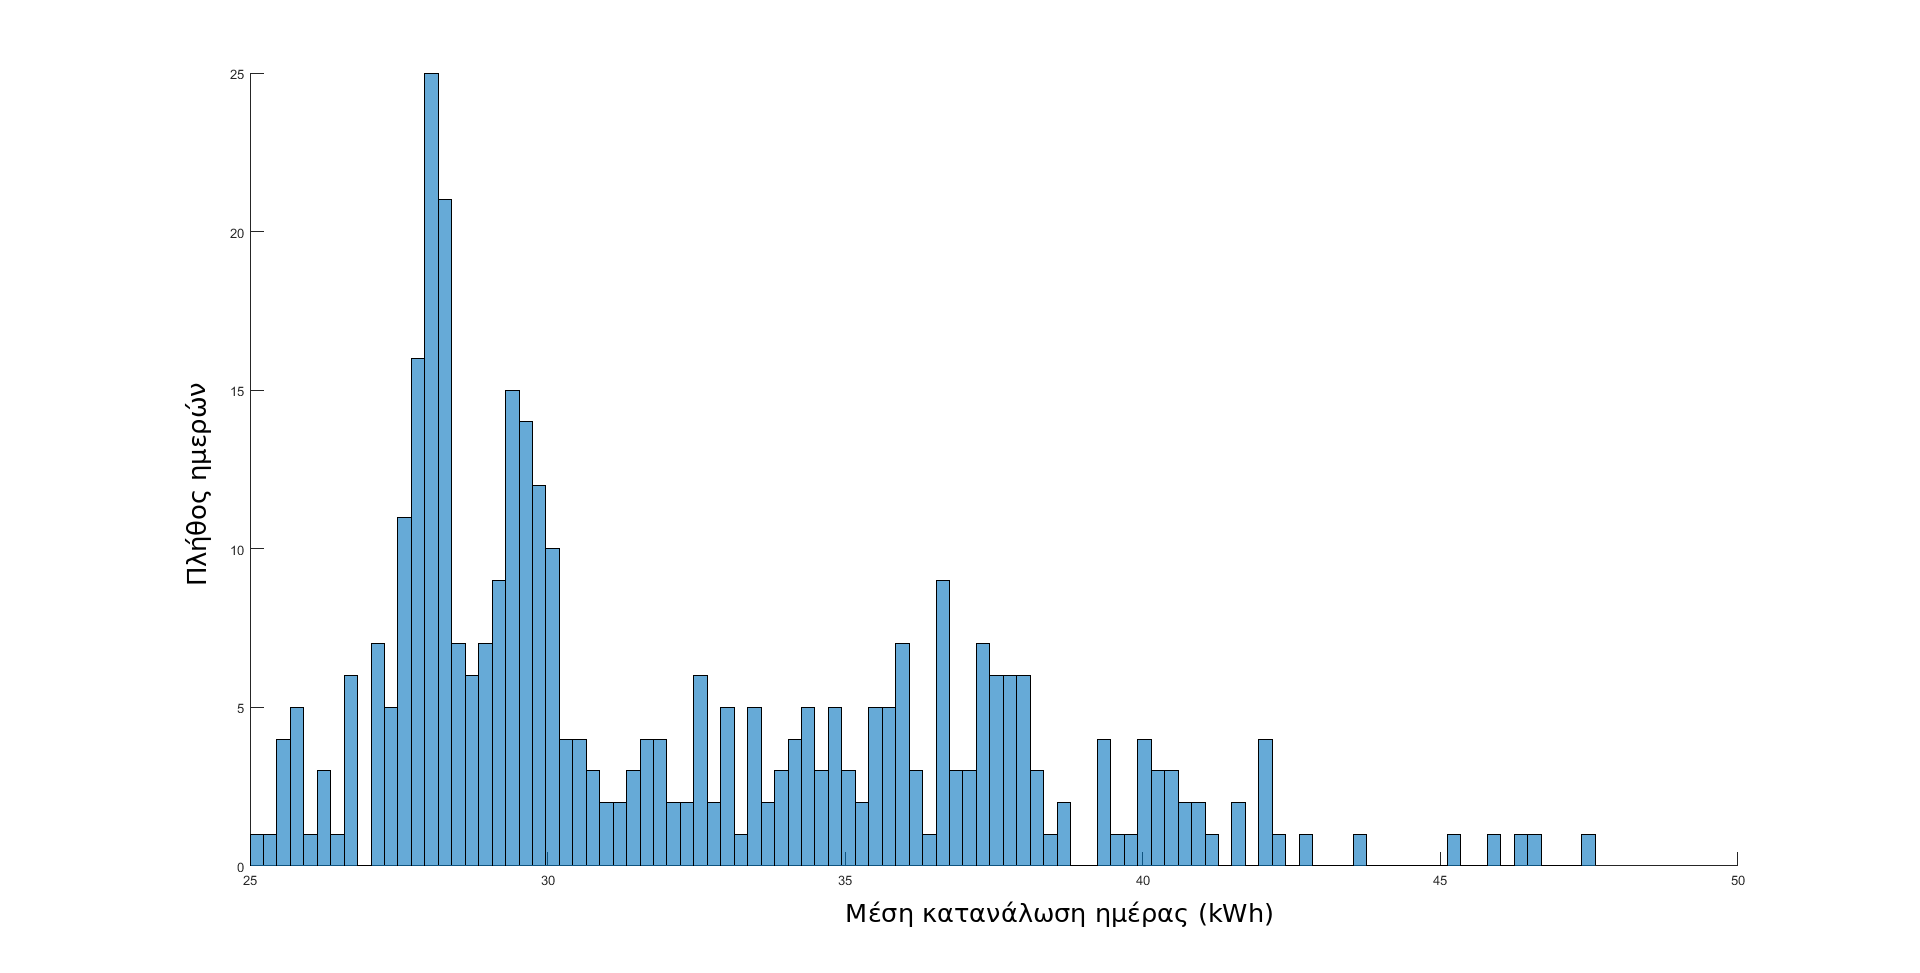
\includegraphics[width=90mm, height=50mm]{../../plots/Consumption_Analysis/gr_hist_mean_days.png}
\caption{Μέσος όρος ημερήσιας κατανάλωσης}
\label{fig:histmeandays}
 \end{subfigure}
\quad
 \begin{subfigure}[b]{0.5\textwidth}
 	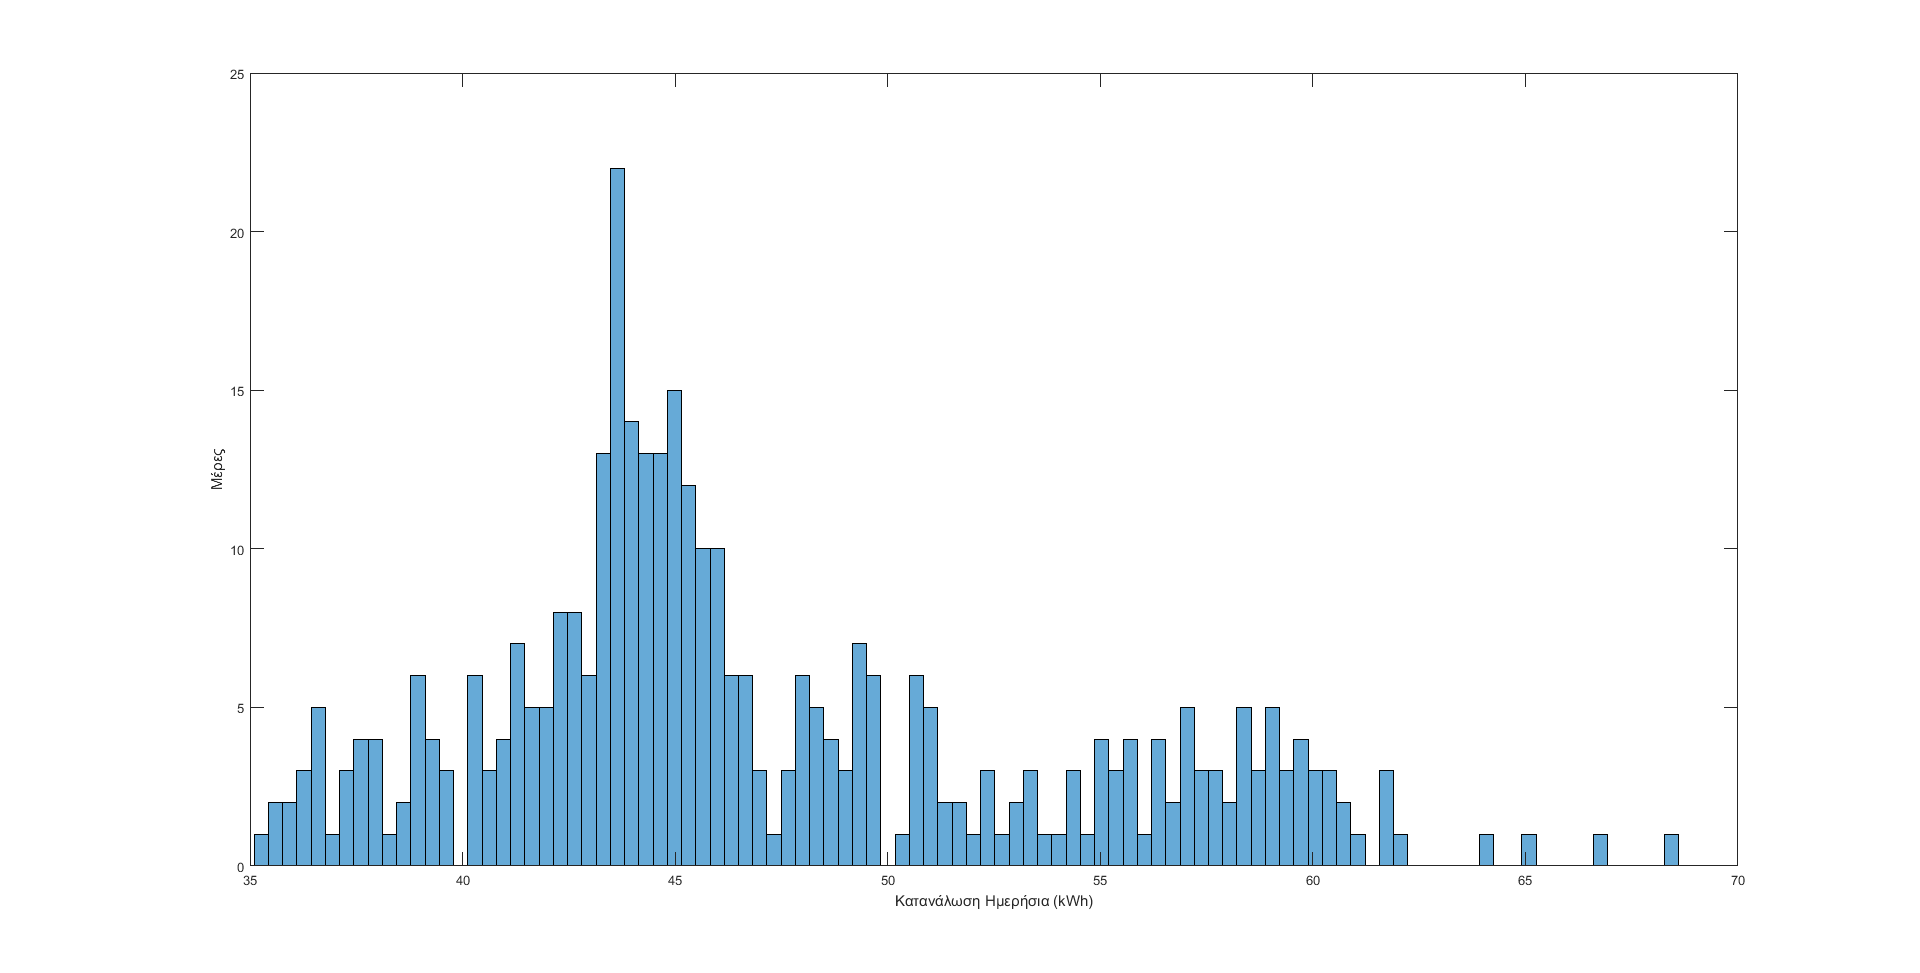
\includegraphics[width=90mm, height=50mm]{../../plots/Consumption_Analysis/gr_hist_std_days.png}
	\caption{Τυπική απόκλιση ημερήσιας κατανάλωσης}
	\label{fig:histstddays}
	\end{subfigure}
\quad
%\centering
 \begin{subfigure}[b]{0.5\textwidth}
 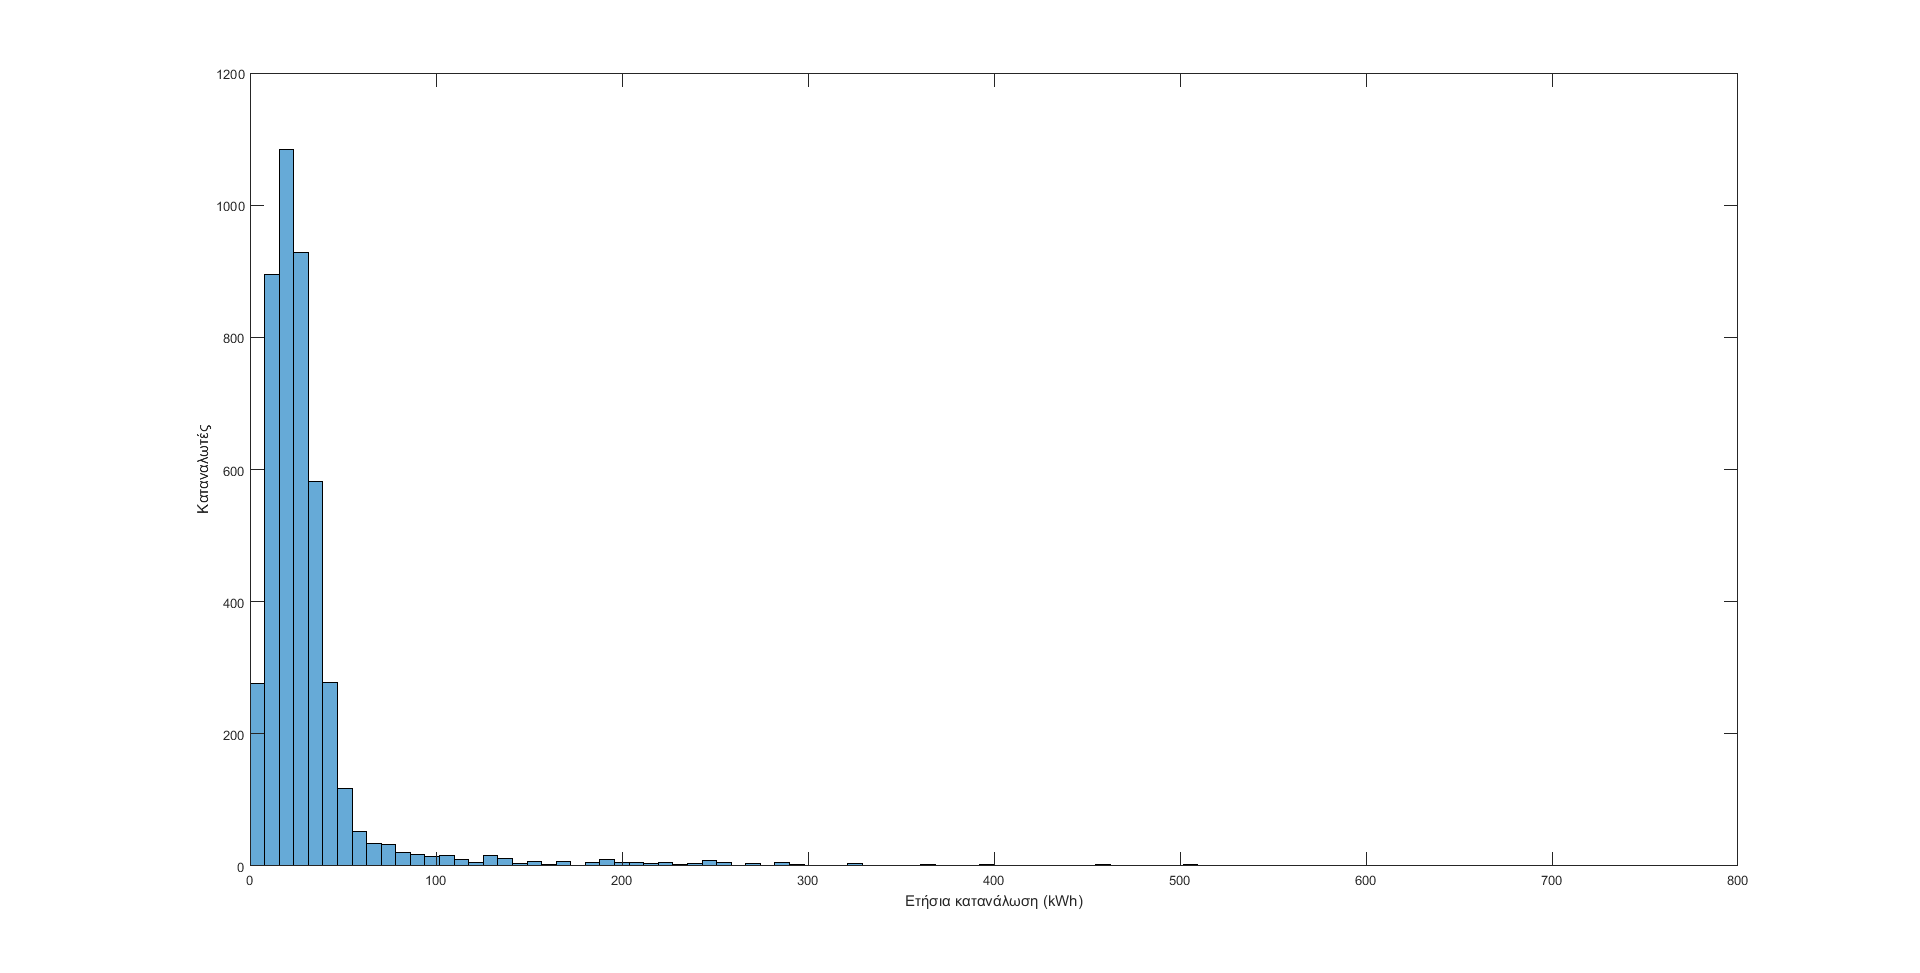
\includegraphics[width=90mm, height=50mm]{../../plots/Consumption_Analysis/gr_hist_mean_year.png}
\caption{Μέσος όρος ετήσιας κατανάλωσης}
\label{fig:histmeanyear}
 \end{subfigure}
\quad
 \begin{subfigure}[b]{0.5\textwidth}
 	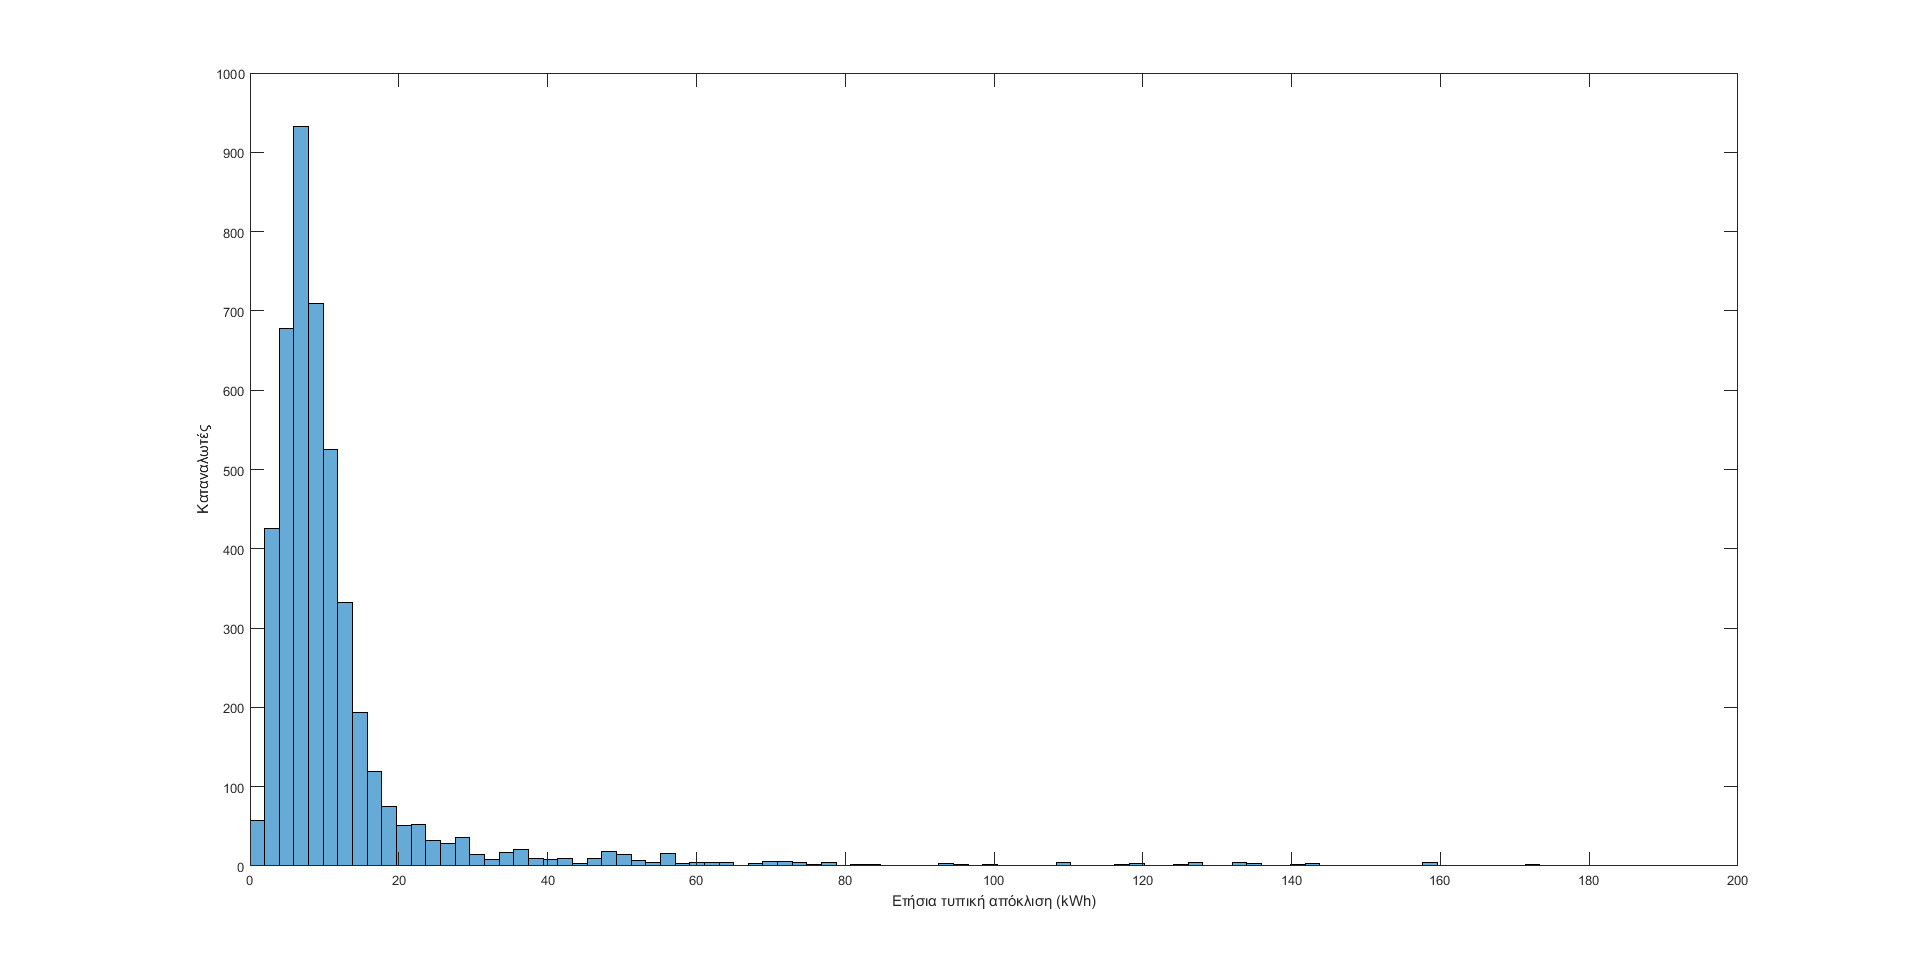
\includegraphics[width=90mm, height=50mm]{../../plots/Consumption_Analysis/gr_hist_std_year.png}
	\caption{Τυπική απόκλιση ετήσιας κατανάλωσης}
	\label{fig:histstdyear}
	\end{subfigure}
	\caption{Ιστογράμματα για καταναλώσεις}
	\label{fig:histograms}
\end{figure}

\begin{figure}
 \begin{subfigure}[b]{0.5\textwidth}
 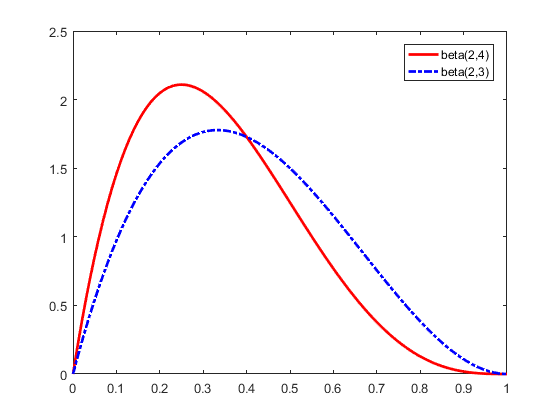
\includegraphics[width=70mm, height=50mm]{../../plots/Consumption_Analysis/beta_days_plot.png}
\caption{Προσέγγιση Βήτα κατανομής στα σχήματα \ref{fig:histmeandays} και \ref{fig:histstddays}}
\label{fig:betadays}
 \end{subfigure}
 \quad
 \begin{subfigure}[b]{0.5\textwidth}
 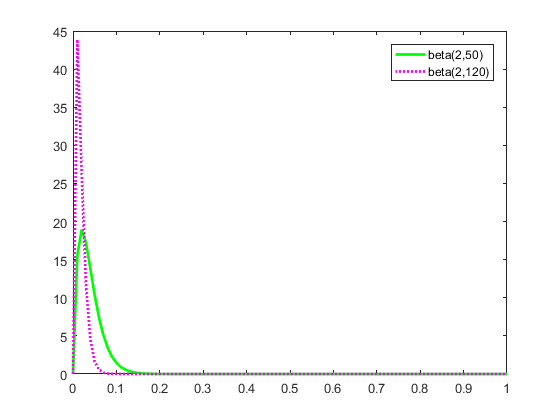
\includegraphics[width=70mm, height=50mm]{../../plots/Consumption_Analysis/beta_year_plot.png}
\caption{Προσέγγιση Βήτα κατανομής στο σχήματα \ref{fig:histmeanyear} και \ref{fig:histstdyear}}
\label{fig:betadays}
 \end{subfigure}
	\caption{Εφαρμογή κατανομής Βήτα}
	\label{fig:betapdfs}
	\end{figure}
\newpage
Γενικότερα, το είδος ασυμμετρίας που ακολουθούν τα ιστογράμματα παρουσιάζουν εξόγκωση προς τα αριστερά και έχουν μεγάλη ουρά προς τα δεξιά ($skewness>0$). Για την προσέγγιση των κατανομών των ιστογραμμάτων χρησιμοποιήθηκε η κατανομή Βήτα, καθώς η συνάρτηση πυκνότητάς της είναι πολύ ευέλικτη στην αναπαράσταση μεγεθών και πιθανοτήτων. Υπάρχουν δύο παράμετροι που θα εργαστούν ταυτοχρόνως για να καθορίσουν αν η κατανομή έχει επικρατούσα τιμή στο διάστημά της και αν αυτή είναι συμμετρική. Η κανονική Βήτα κατανομή παρέχει την πυκνότητα πιθανότητας της τιμής $x$ στο διάστημα(0,1):
\begin{center}
$Beta(\alpha, \beta):prob(x\|\alpha, \beta)=\frac{x^{\alpha-1}(1-x)^{\beta-1}}{B(\alpha, \beta)}$
\end{center}
όπου $B$ είναι η βήτα συνάρτηση
\begin{center}
$Β(\alpha, \beta)=\int_{0}^{1} t^{\alpha-1}(1-t)^{\beta-1}dt$
\end{center}
Για την προσέγγιση των σχημάτων \ref{fig:histmeandays} και \ref{fig:histstddays} χρησιμοποιήθηκαν οι κατανομές $Beta(2,4)$ και $Beta(2,3)$, ενώ τα σχήματα \ref{fig:histmeanyear} και \ref{fig:histstdyear} αντιστοιχίζονται με τις κατανομές $Beta(2,50)$ και $Beta(2,120)$ δημιουργώντας σε κάθε παράδειγμα μια επικρατούσα τιμή. Παρακάτω μπορεί να φανεί η αναπαράστασή τους στο Σχήμα \ref{fig:betapdfs}.

\begin{table}
\begin{tabular}{ |c|c|c|c|c| }
 \hline
 Μέτρο & Σχήμα \ref{fig:histmeandays} & Σχήμα \ref{fig:histstddays} & Σχήμα \ref{fig:histmeanyear} & Σχήμα \ref{fig:histstdyear}\\
 \hline
 Μέσος Όρος   		&   31.99  & 42.61 &31.99 &12.4111\\
 \hline
  Διάμεσος   		&   29.82  & 40.24 &23.85 &8.34\\ 
  \hline
  Επικρατούσα Τιμή  &   24.71  & 30.44 &23.50&9.95\\ 
   \hline
\end{tabular}
\caption{Ποσοτικά μέτρα περιγραφής ιστογραμμάτων}
\label{tab:metricshist}
\end{table}

Ένα ακόμη απαραίτητο στάδιο στη μελέτη ιστογραμμάτων θετικής λοξότητας είναι η ποσοτικοποίηση μετρικών που να συνοψίζουν τα δεδομένα. Για αυτό το στάδιο επιλέχθηκαν ο μέσος όρος, ο διάμεσος και η επικρατούσα τιμή. Τα αποτελέσματα για κάθε ιστόγραμμα μπορούν να φανούν στον Πίνακα \ref{tab:metricshist}.
\subsection{Μοντελοποίηση εποχιακών δεικτών}
Για βαθύτερη κατανόηση των χρονοσειρών γίνεται εκτίμηση της εποχιακής και μη εποχιακής καταναλωτικής τάσης με τη χρήση παραμετρικών μοντέλων. Με αυτό τον τρόπο θα καταστεί δυνατή η παρατήρηση της επαναληψιμότητας και των μορφών των καταναλώσεων. Για να γίνει αυτό χρησιμοποιείται αρχικά ο αλγόριθμος \en{K-Means} για την ομαδοποίηση των καταναλωτών σε τέσσερις συστάδες βάση του ετήσιου μέσου όρου καθενός. Στη συνέχεια δημιουργείται ένα προφίλ κατανάλωσης για κάθε συστάδα βρίσκοντας το μέσο ημερήσιο όρο κατανάλωσης. Χρειάστηκαν 2000 καταναλωτές για αυτή την ανάλυση με περισσότερους  1800 να ομαδοποιούνται σε δύο ομάδες υποδεικνύοντας προφίλ οικιακών καταναλωτών.
\subsubsection{Ανάλυση Παλινδρόμησης}
Σκοπός, λοιπόν αυτού του μέρους είναι να γίνει στατιστική μελέτη του πολυωνυμικού μοντέλου στα δεδομένα μας και να δούμε αν οι χρονοσειρές κάθε συστάδας μπορούν να περιγραφούν  με πολυώνυμο δευτέρου βαθμού. \cite{mathworkstrend}
\begin{center}
$T_t=\beta_0 + \beta_1t + \beta_2t^2$
\end{center}

\begin{figure}[ht!]
\centering
\includegraphics[width=180mm, height=120mm]{../../plots/Trend_estimation/quadratic_Trend_ALL.png}
\caption{Εφαρμογή πολυωνύμου δευτέρου  βαθμού}
\label{fig:quadratic trend}
\end{figure}


Όπως φαίνεται στο Σχήμα \ref{fig:quadratic trend} οι συστάδες μπορούν να χαρακτηριστούν από μια παραβολική καμπύλη με θετικό συντελεστή μεγιστοβάθμιου όρου.
\begin{itemize}
\item Η συστάδα 1 αποτελείται από 792 καταναλωτές και έχει η παραβολική καμπύλη τάσης λαμβάνει ελάχιστη τιμή την 189η μέρα του έτους.
\item Η συστάδα 2 αποτελείται από 81 καταναλωτές και έχει η παραβολική καμπύλη τάσης λαμβάνει ελάχιστη τιμή την 206η μέρα του έτους. 
\item Η συστάδα 3 αποτελείται από 81 καταναλωτές και έχει η παραβολική καμπύλη τάσης λαμβάνει ελάχιστη τιμή την 201η μέρα του έτους.
\item Η συστάδα 4 αποτελείται από 81 καταναλωτές και έχει η παραβολική καμπύλη τάσης λαμβάνει ελάχιστη τιμή την 194η μέρα του έτους.
\end{itemize}

Εύκολα, λοιπόν, βγάνει το συμπέρασμα πως οι οικιακοί καταναλωτές έχουν την τάση να έχουν πιο ομοιόμορφα κατανεμημένα την παραβολική καμπύλη, ενώ οι επιχειρήσεις έχουν μεγαλύτερο βαθμό τυχαιότητας και λιγότερο συμμετρική καμπύλη ως προς το ελάχιστο σημείο της.
\subsubsection{Εκτίμηση εποχιακών δεικτών}
Αρχικά για την εκτίμηση των εποχιακών δεικτών απαιτείται η αφαίρεση του πολυώνυμου δευτέρου βαθμού από τις χρονοσειρές των ομάδων.\cite{timeseriesanalysis} Δεδομένης της μικρής διάρκειας των καταναλώσεων (1 έτος) καθίσταται αδύνατη η εξαγωγή εποχιακών δεικτών ανά μήνα έτους ή ανά εποχή έτους. Για αυτό το λόγο οι εποχιακοί δείκτες μεταφέρθηκαν ανά ημέρα της εβδομάδας ή ανά ημέρα του μήνα. Για την πρώτη περίπτωση οι δείκτες αναφέρονται στις ημέρες κάθε εβδομάδας, ενώ για την δεύτερη αναφέρονται στις ημέρες κάθε μήνα δημιουργώντας 7 ή 30 δείκτες αντίστοιχα. Για την εβδομαδιαία εποχιακότητα έχω τις παρακάτω καμπύλες για κάθε ομάδα.
\subsubsection{Εκτίμηση με διαστήματα ημέρας ανά εβδομάδα}
Από την εβδομαδιαία εποχιακότητα λοιπόν εύκολα κάποιος αντιλαμβάνεται πως ανάλογα με τον τύπο των καταναλωτών οι μέρες που έχουμε μέγιστη και ελάχιστη κατανάλωση διαφέρουν ριζικά. Η πρώτη μέρα του έτους για το έτος που μελετάμε είναι Πέμπτη. Ειδικότερα:
\begin{itemize}
\item Για τους καταναλωτές συστάδας 1 (οικιακοί καταναλωτές) έχουμε ελάχιστες καταναλώσεις τις Πέμπτες.
\item Για τους καταναλωτές συστάδας 2 (επιχειρήσεις) έχουμε ελάχιστες καταναλώσεις τα Σάββατα.
\item Για τους καταναλωτές συστάδας 3 (οικιακοί καταναλωτές) έχουμε ελάχιστες καταναλώσεις τις Τρίτες.
\item Για τους καταναλωτές συστάδας 4 (επιχειρήσεις) έχουμε ελάχιστες καταναλώσεις τα Σάββατα.
\end{itemize}
\newpage
\begin{figure}[ht!]
\centering
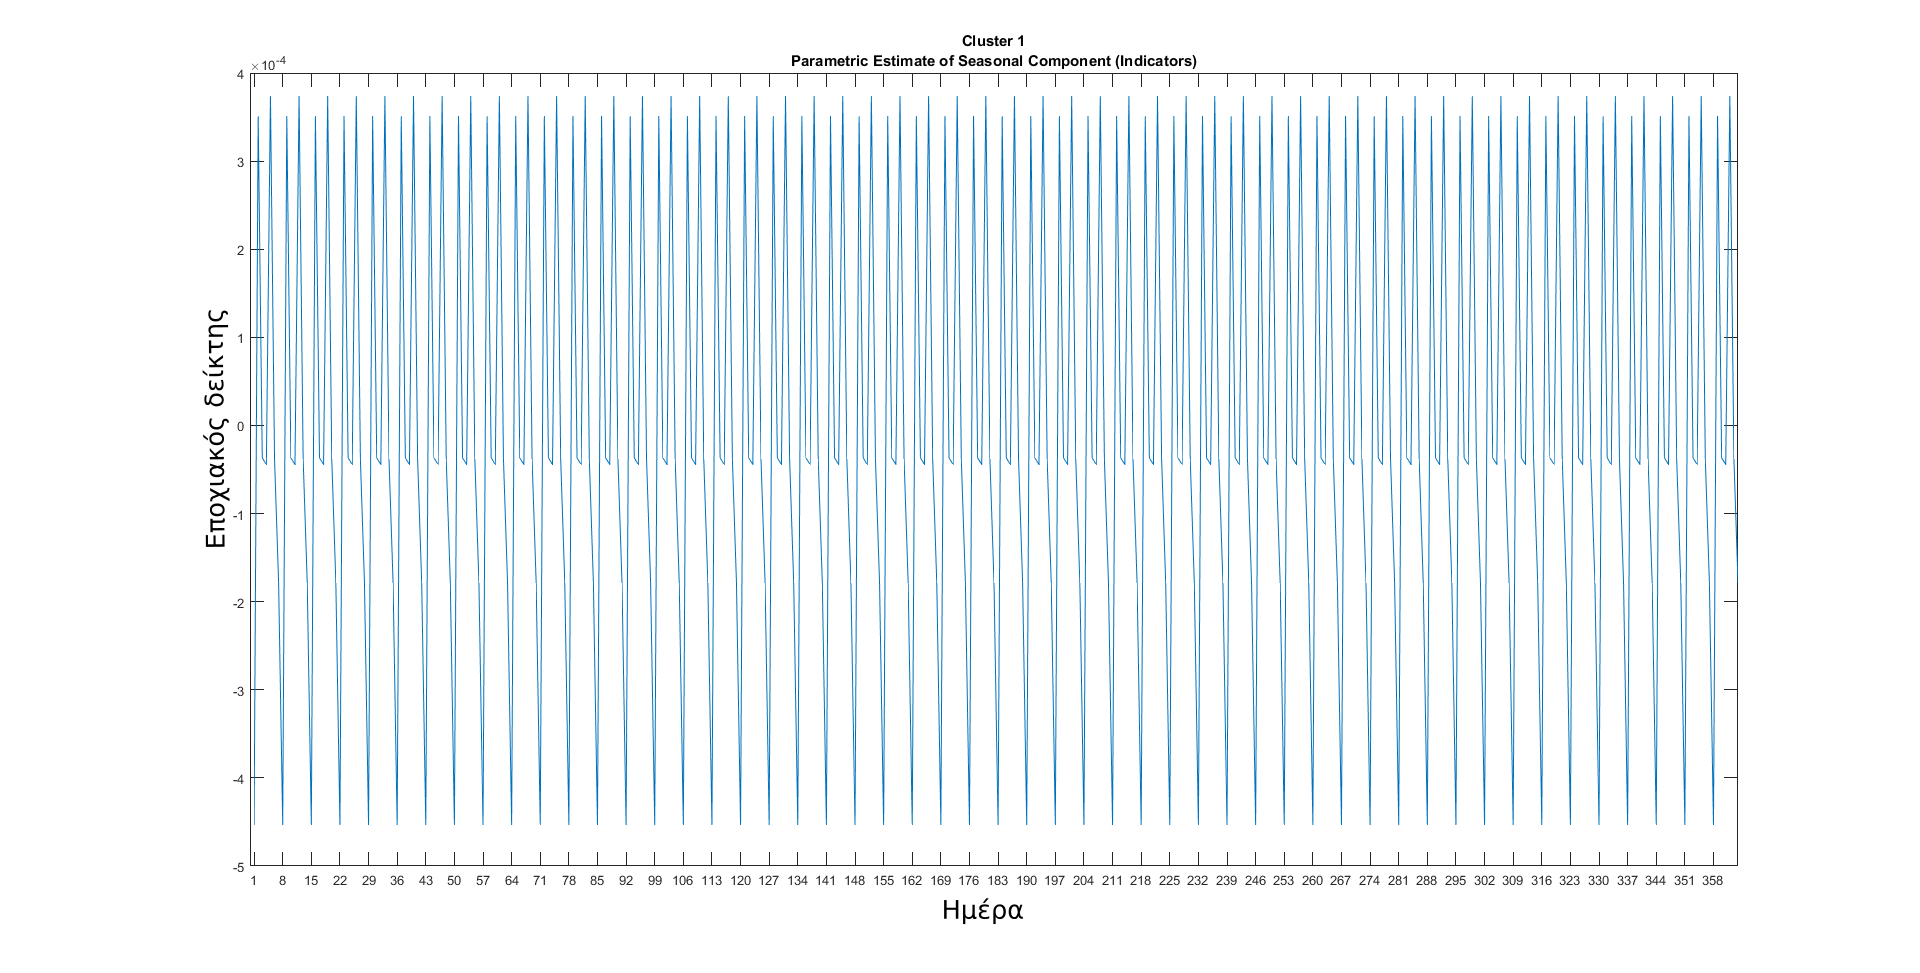
\includegraphics[width=180mm, height=100mm]{../../plots/Trend_estimation/seasonal_1.png}
\caption{Εβδομαδιαία εποχιακότητα ομάδας 1}
\label{fig:season 1}
\end{figure}
\begin{figure}[ht!]
\centering
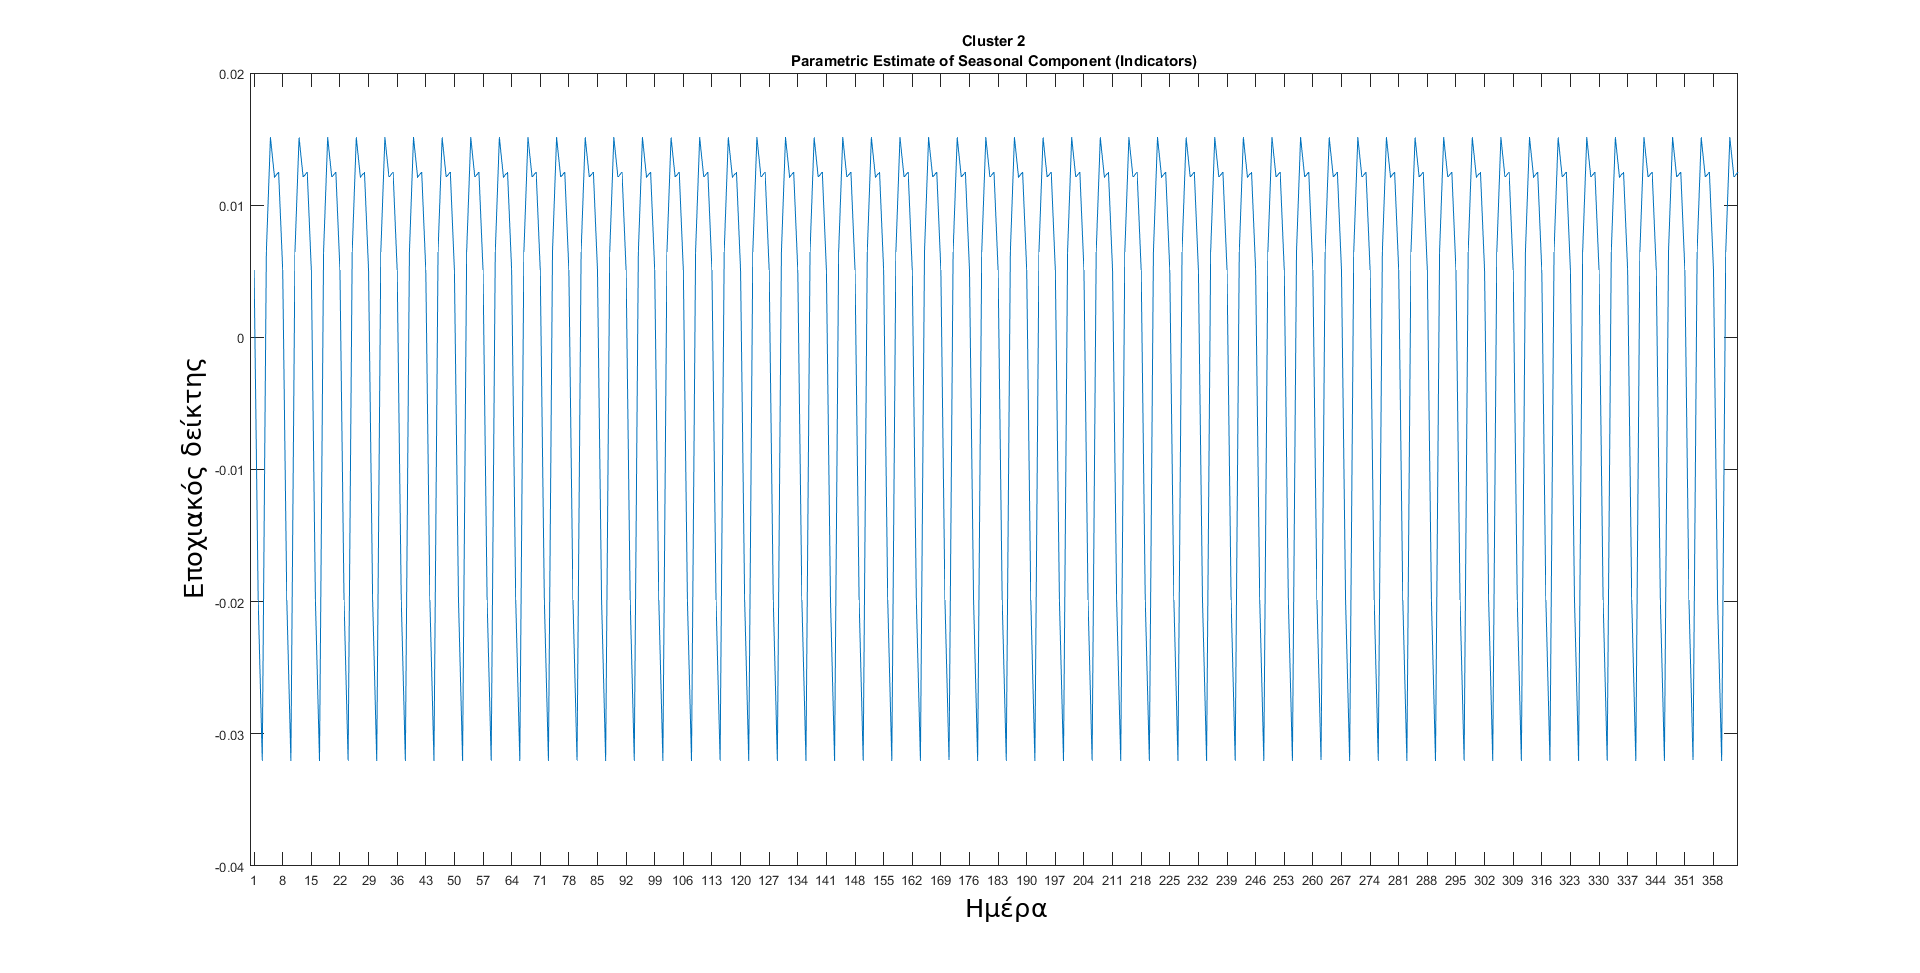
\includegraphics[width=180mm, height=100mm]{../../plots/Trend_estimation/seasonal_2.png}
\caption{Εβδομαδιαία εποχιακότητα ομάδας 2}
\label{fig:season 2}
\end{figure}
\begin{figure}[ht!]
\centering
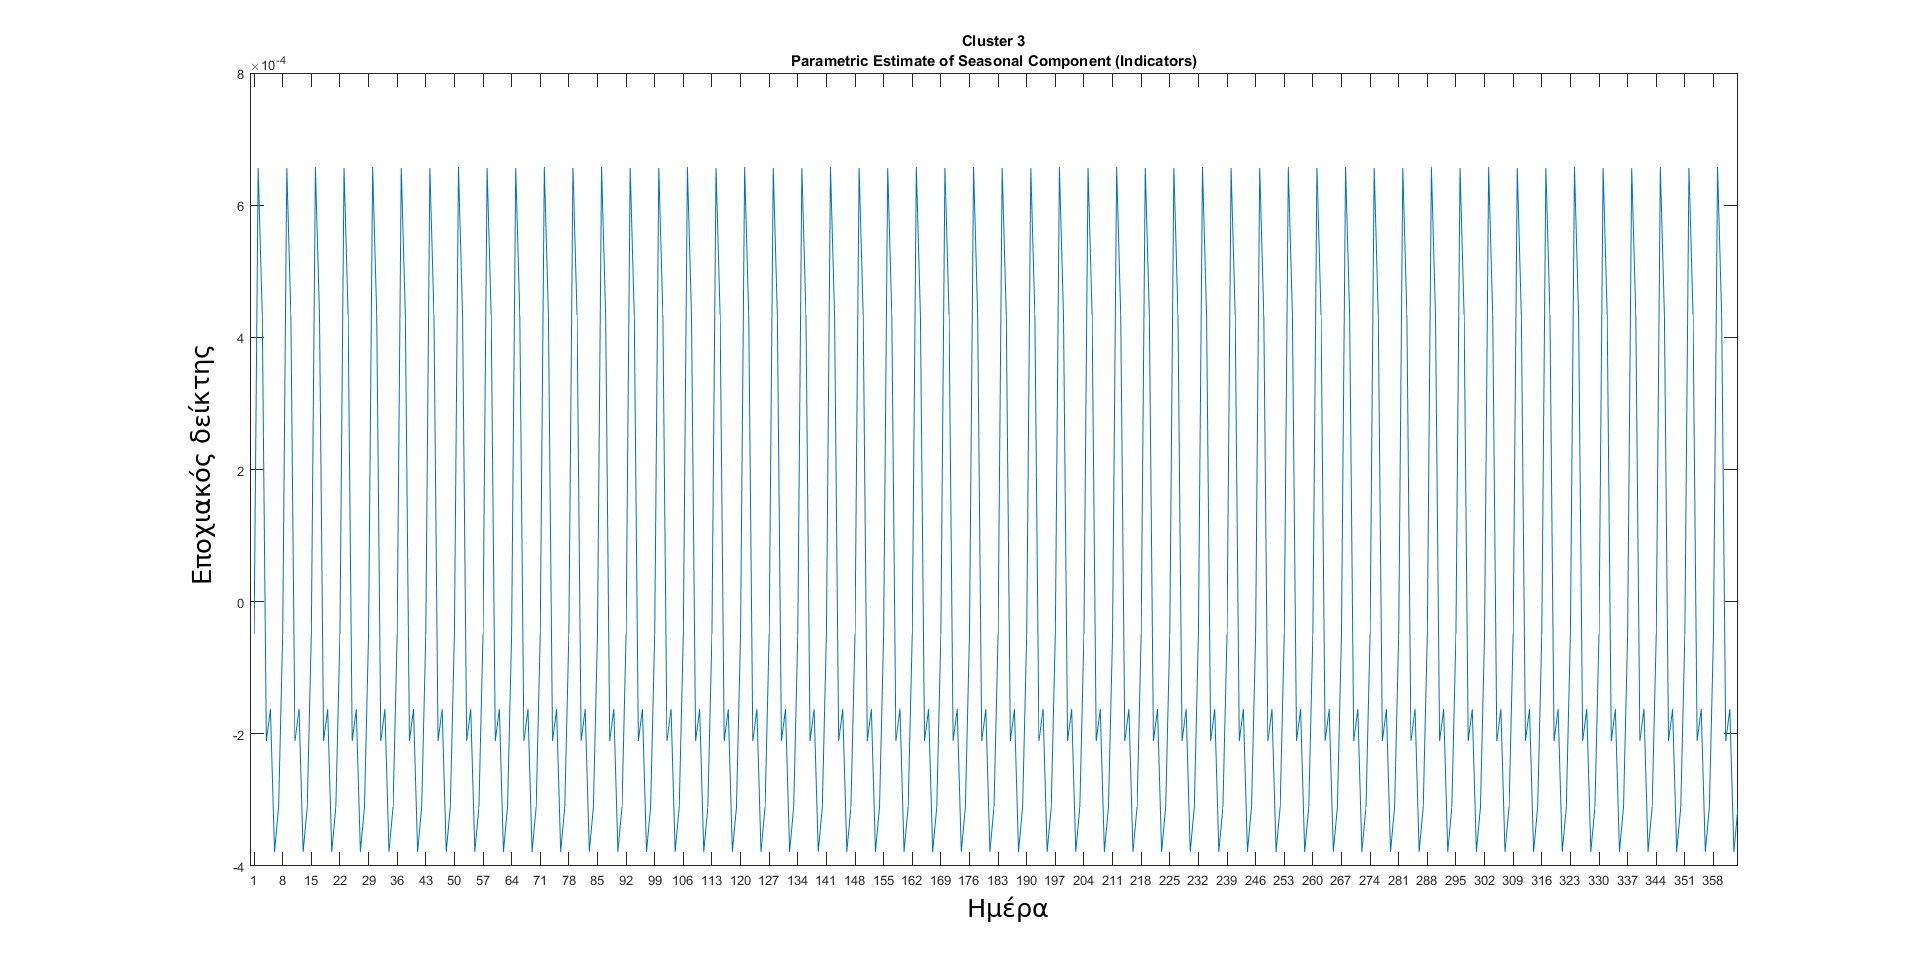
\includegraphics[width=180mm, height=100mm]{../../plots/Trend_estimation/seasonal_3.png}
\caption{Εβδομαδιαία εποχιακότητα ομάδας 3}
\label{fig:season 3}
\end{figure}
\begin{figure}[ht!]
\centering
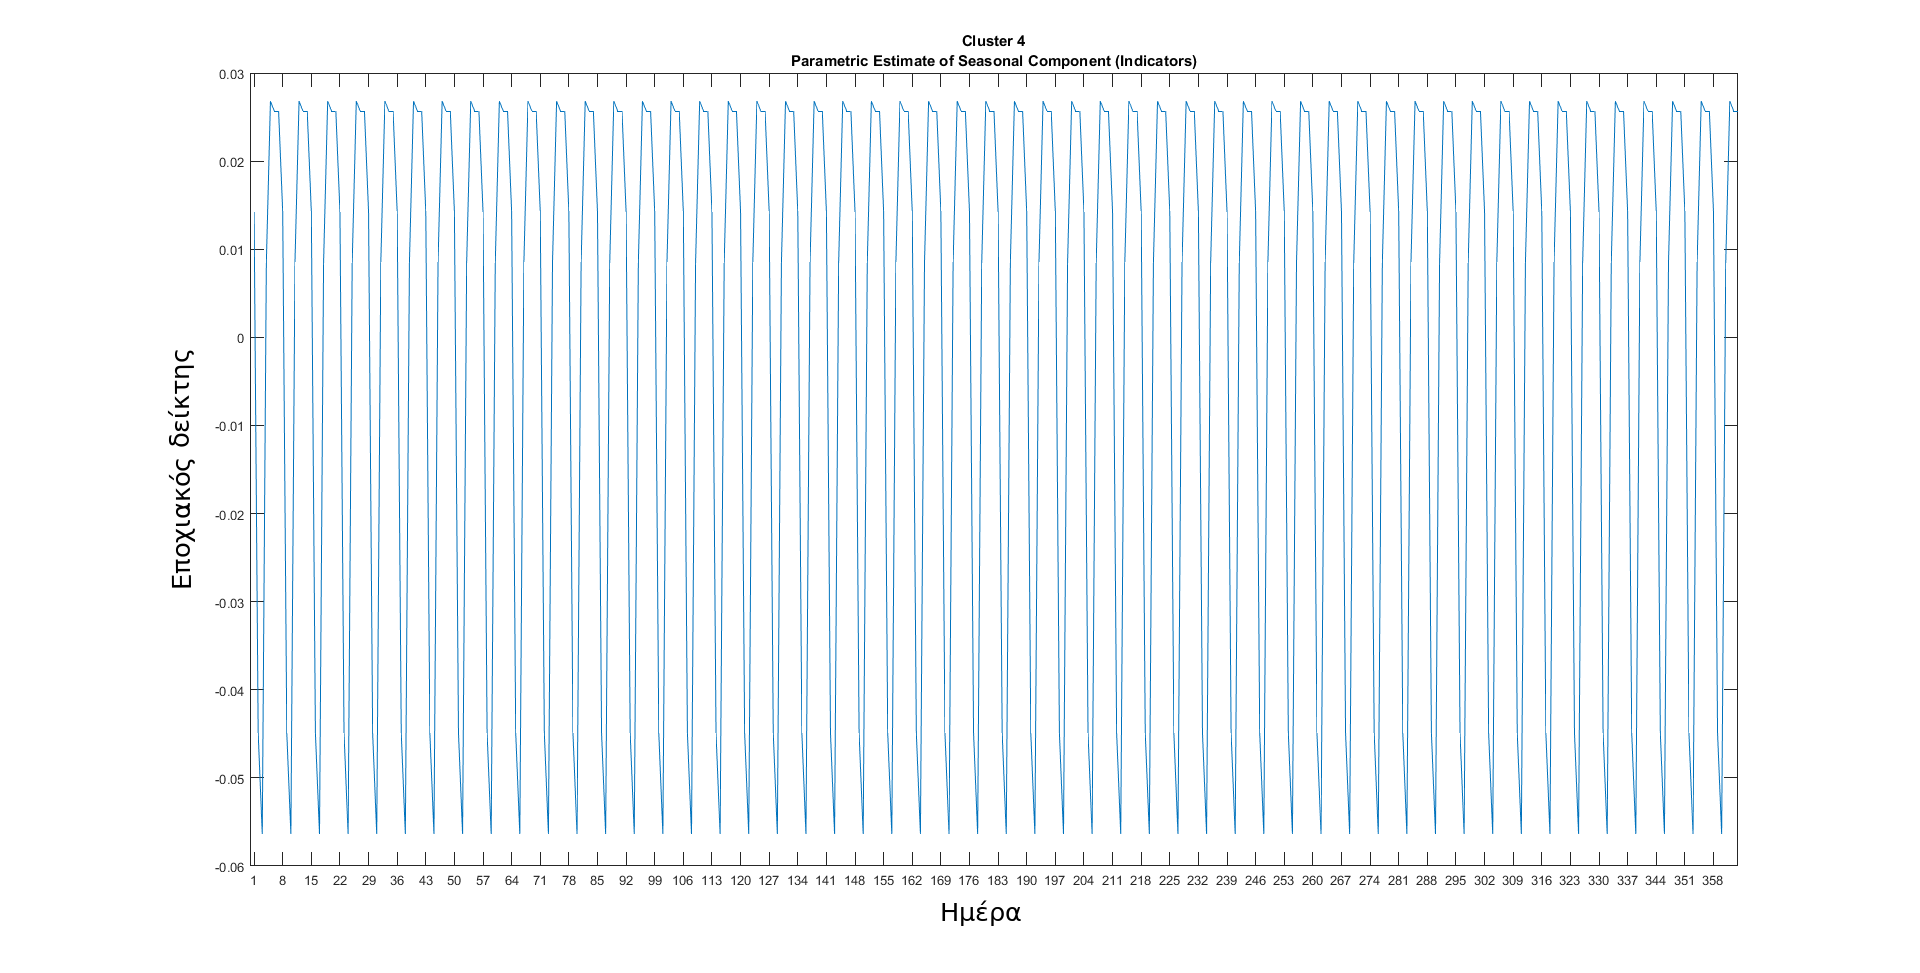
\includegraphics[width=180mm, height=100mm]{../../plots/Trend_estimation/seasonal_4.png}
\caption{Εβδομαδιαία εποχιακότητα ομάδας 4}
\label{fig:season 4}
\end{figure}
\subsubsection{Εκτίμηση σε διαστήματα ημέρας ανά μήνα}
Το διάστημα ενός μήνα αφήνει μεγαλύτερα περιθώριο εποπτείας της χρονοσειράς, ενώ ταυτόχρονα δημιουργεί αποτελέσματα με μεγαλύτερη συνοχή. Από την άλλη πλευρά οι 12 μήνες του έτους δεν μπορούν να εξάγουν πολύ ασφαλή δεδομένα αν συγκριθούν με τις 52 εβδομάδες.


Από την μηνιαία εποχιακότητα γίνεται εύκολα αντιληπτό πως ανάλογα με τον τύπο των καταναλωτών οι μέρες που έχουμε μέγιστη και ελάχιστη κατανάλωση διαφέρουν ριζικά. Ειδικότερα:
\begin{itemize}
\item Για τους καταναλωτές συστάδας 1 (επιχειρήσεις) έχουμε ελάχιστες καταναλώσεις στις 30 του μηνός.
\item Για τους καταναλωτές συστάδας 2 (οικιακοί καταναλωτές) έχουμε ελάχιστες καταναλώσεις στις 15 του μηνός.
\item Για τους καταναλωτές συστάδας 3 (οικιακοί καταναλωτές) έχουμε ελάχιστες καταναλώσεις στις 15 του μηνός.
\item Για τους καταναλωτές συστάδας 4 (επιχειρήσεις) έχουμε ελάχιστες καταναλώσεις στις 3 του μηνός.
\end{itemize}
\begin{figure}[ht!]
\centering
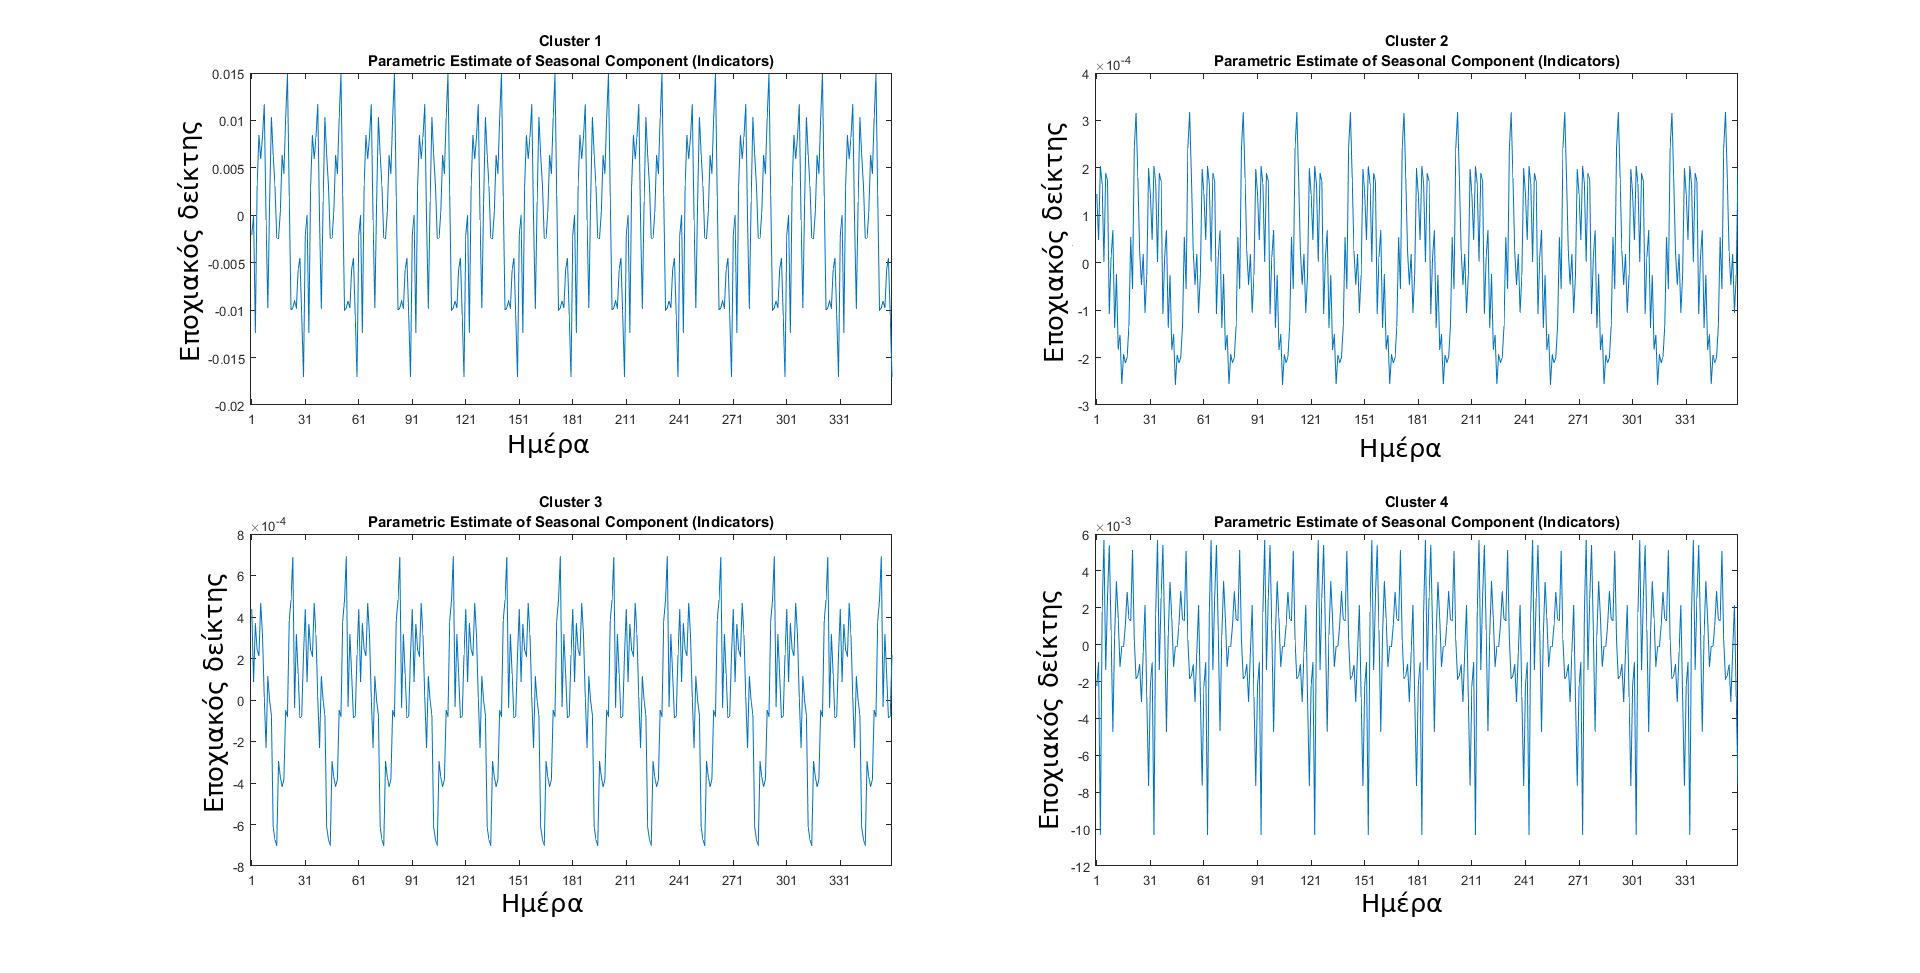
\includegraphics[width=180mm, height=120mm]{../../plots/Trend_estimation/seasonal_month_ALL.png}
\caption{Μηνιαία εποχιακότητα}
\label{fig:season daypermonth}
\end{figure}
\subsubsection{Αφαίρεση εποχιακών δεικτών}
Σε αυτό το σημείο είναι σημαντικό να παρατηρηθεί η κατανάλωση χωρίς τους εποχιακούς δείκτες. Με αυτό τον τρόπο καθίσταται ευκολότερη η θεώρηση της μορφής των κυματομορφών και η σύγκρισή τους με τις αρχικές καταναλώσεις του πρώτου μέρους. Αφαιρώντας τα εποχιακά χαρακτηριστικά οι καμπύλες πλησιάζουν περισσότερο στην παραβολική συνάρτηση. Έτσι η καταναλωτική τους τάση χωρίς τους εποχιακούς δείκτες γίνεται πιο έντονη και ευδιάκριτη.
\begin{figure}[ht!]
\centering
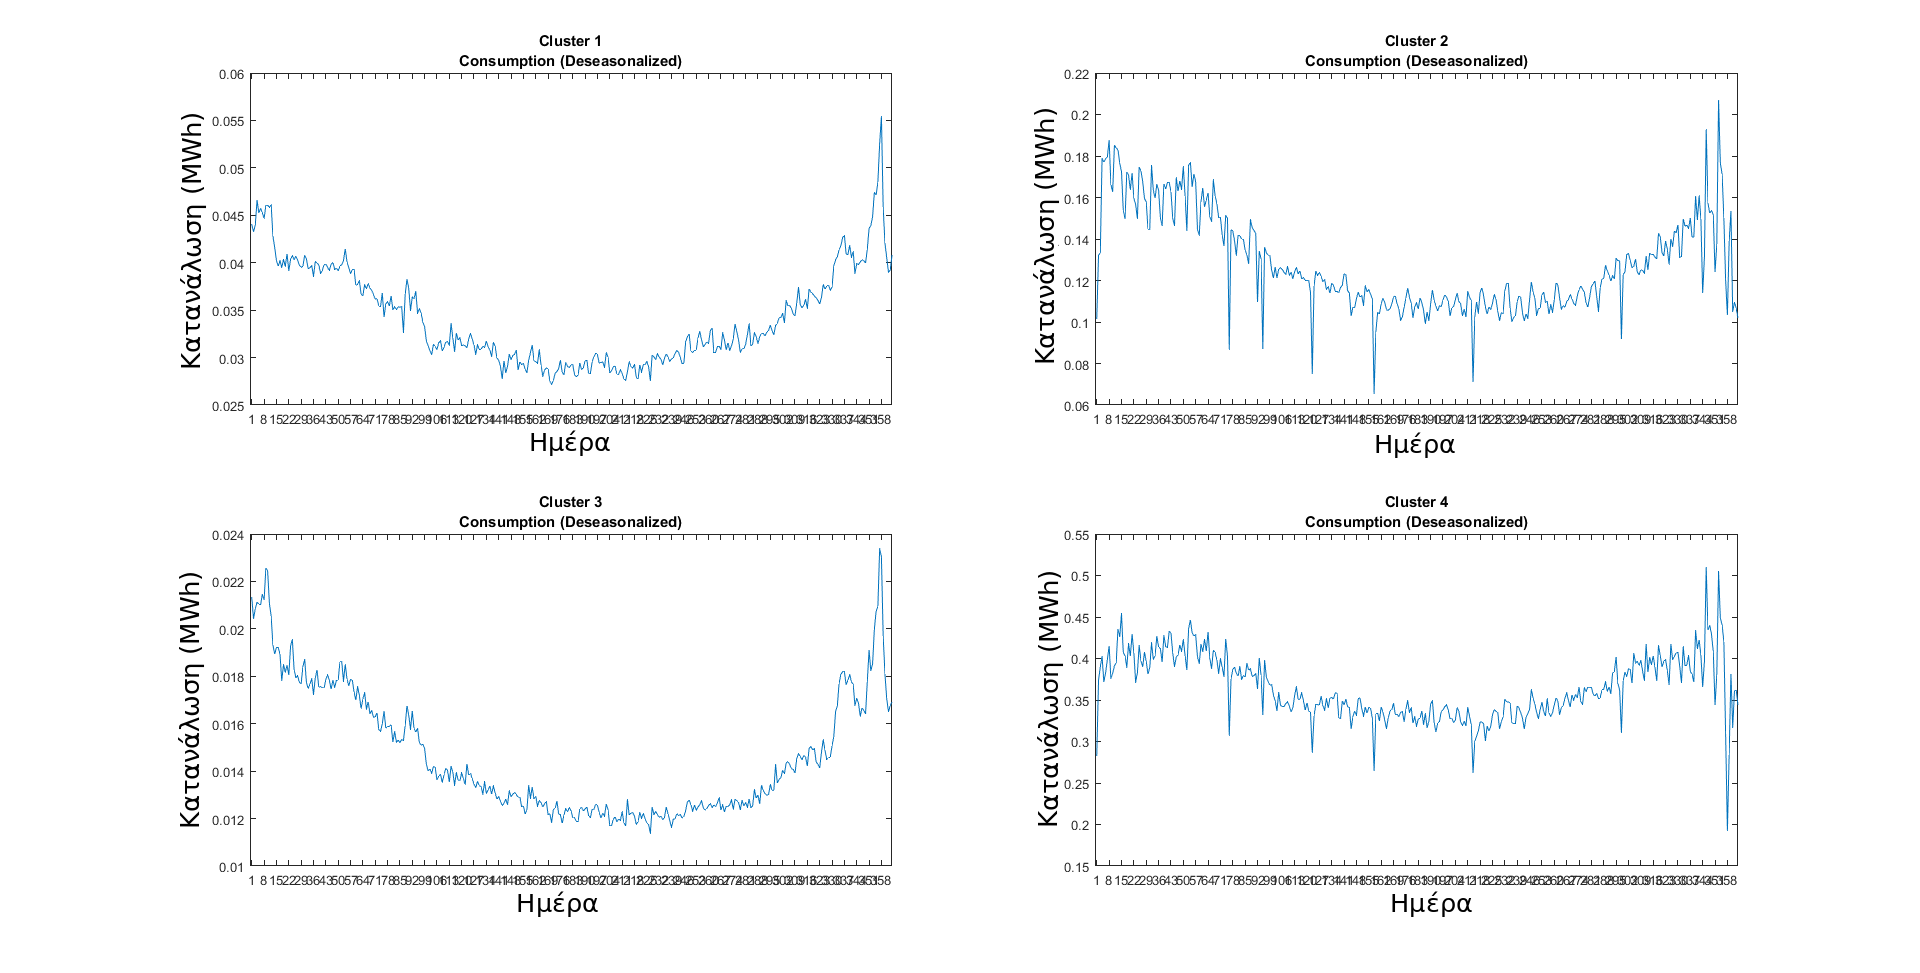
\includegraphics[width=180mm, height=120mm]{../../plots/Trend_estimation/Deseasonalized_ALL.png}
\caption{Κατανάλωση χωρίς εποχιακούς δείκτες ανά εβδομάδα}
\label{fig:deseason week}
\end{figure}
\newpage

\begin{figure}[ht!]
\centering
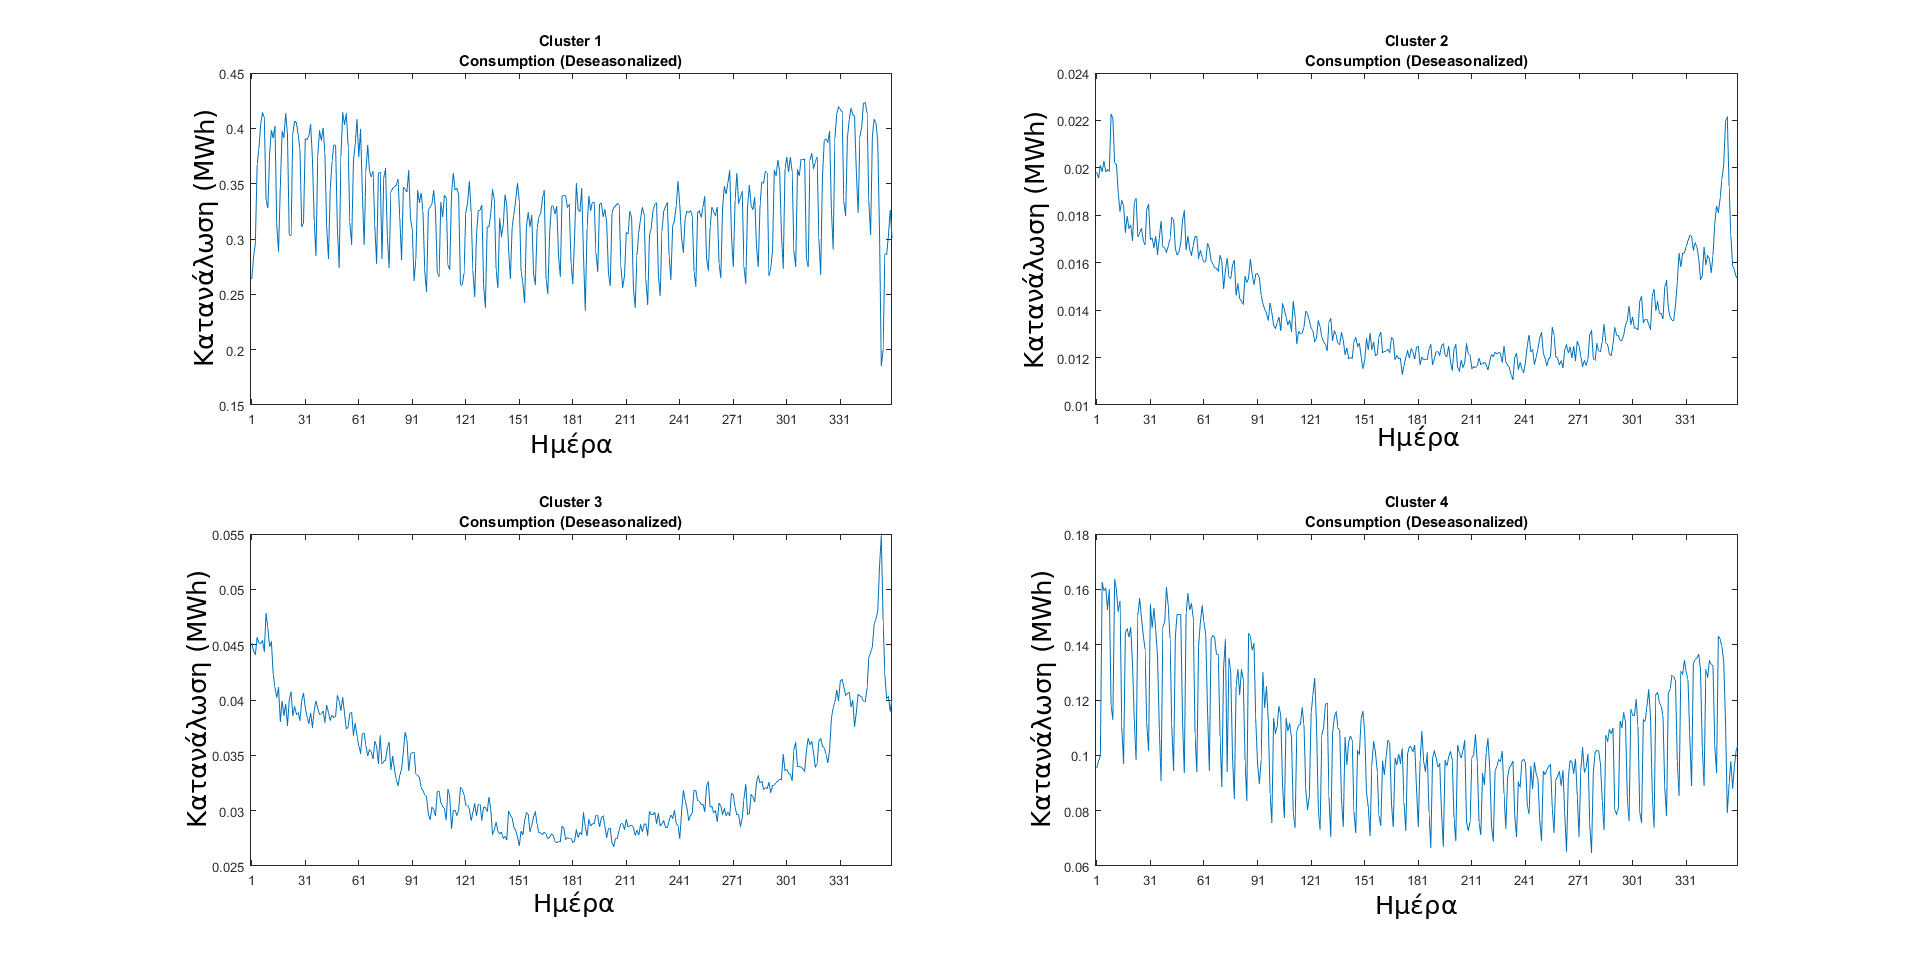
\includegraphics[width=180mm, height=120mm]{../../plots/Trend_estimation/Deseasonalized_month_ALL.png}
\caption{Κατανάλωση χωρίς εποχιακούς δείκτες ανά μήνα}
\label{fig:deseason month}
\end{figure}

\subsubsection{Εκτίμηση ακανόνιστης συνιστώσας}
Τέλος έχει ενδιαφέρουν να δούμε το βαθμό της τυχαιότητας που έχουμε στις καταναλώσεις των συστάδων που δημιουργήθηκαν. Αυτό επιτυγχάνεται αφαιρώντας την εποχιακή χρονοσειρά και την καταναλωτική τάση της αρχικής χρονοσειράς. Με αυτό τον τρόπο γίνεται σαφές ότι παρόλο την εποχιακότητα και την τάση οι χρονοσειρές έχουν αισθητό τυχαίο παράγοντα. Η αφαίρεση δημιουργεί αλλαγές στο επίπεδο της χεονοσειράς, σταθεροποιώντας έτσι το μέσο όρο της. Γίνεται αντιληπτό πως έχουν μη προβλέψιμα πρότυπα  τουλάχιστον με δεδομένα διάρκειας ενός έτους. Τέτοιου τύπου δεδομένα λέγενται στατικές χρονοσειρές.\cite{stationarity}
\begin{figure}[ht!]
\centering
\includegraphics[width=180mm, height=100mm]{../../plots/Trend_estimation/irregular_component_all.png}
\caption{Εκτίμηση ακανόνιστης συνιστώσας με εβδομαδιαία εποχιακότητα}
\label{fig:irregular week}
\end{figure}

\newpage
\begin{figure}[ht!]
\centering
\includegraphics[width=180mm, height=100mm]{../../plots/Trend_estimation/irregular_component_month_all.png}
\caption{Εκτίμηση ακανόνιστης συνιστώσας με μηνιαία εποχιακότητα}
\label{fig:irregular month}
\end{figure}
\subsubsection{Εξερεύνηση ημερών με χαμηλές καταναλώσεις}
Για να αντληθούν περαιτέρω χαρακτηριστικά των χρονοσειρών χρειάστηκε η υλοποίηση αλγορίθμου με διπλή συσταδοποίηση. Σύμφωνα με τον αλγόριθμο πρώτα συσταδοποιούνται οι καταναλωτές με βάση την ημερήσια κατανάλωση, εν συνεχεία για κάθε συστάδα δημιουργείται νέα ομαδοποίηση με βάση την ομοιότητα κάθε ημερήσιας κατανάλωσης. Με αυτό τον τρόπο μπορεί να παρατηρηθεί ποιες μέρες όμοιων καταναλωτών έχουν παρόμοιες καταναλώσεις. Καθίσταται έτσι εφικτό, να φιλτράρουμε από τα δεδομένα μας μέρες με χαμηλή κατανάλωση που γνωρίζουμε πως θα δυσκόλευαν το πρόβλημα της ταξινόμησης σε αληθή και αλλοιωμένα δεδομένα.

Τα αποτελέσματα του αλγορίθμου έδειξαν πως μόνο τα Σάββατα μιας συστάδας εμφανίζουν έντονη ομοιότητα οικιακών καταναλώσεων. Οι Κυριακές κατά κύριο λόγο συσταδοποιούνται με την υπόλοιπη εβδομάδα δημιουργώντας την εβδομαδιαία τάση, γεγονός που δείχνει πως για τους περισσότερους καταναλωτές η Κυριακή είναι εργάσιμη ημέρα. Παράλληλα, παρατηρείται πως ανά περιόδους οι καταναλώσεις δημιουργούν νέες συστάδες αφήνοντας μόνο τα Σάββατα να σπάνε την συνεχόμενη συσταδοποίηση. Στον Πίνακα \ref{tab:double clustering} φαίνεται πως ακόμη και στα Σάββατα δεν έχουμε απολύτως γεμάτες συστάδες.

\begin{table}[ht!]
\centering
\begin{tabular}{ |c||c|c|c|c|  }
 \hline
 \multicolumn{5}{|c|}{Συστάδες Καταναλωτών} \\
 \hline
 Συστάδες Σαββάτου  & Συστάδα 1& Συστάδα 2 &Συστάδα 3 &Συστάδα 4\\
 \hline
 Συστάδα 1 & 0  & 24 & 30 & 19\\
 Συστάδα 2 & 9  & 11 & 0  & 15\\
 Συστάδα 3 & 0  & 9  & 0  & 0\\
 Συστάδα 4 & 42 & 0  & 0  & 0\\
 Συστάδα 5 & 0  & 2  & 0  & 0\\
 Συστάδα 6 & 0  & 4  & 0  & 7\\
 Συστάδα 7 & 0  & 1  & 21 & 10\\
 \hline
\end{tabular}
\caption{Έλεγχος συσταδοποίησης Σαββάτου}
\label{tab:double clustering}
\end{table}

\subsubsection{Παρατηρήσεις}
Τα εμφανή χαρακτηριστικά εποχιακότητας και η εφαρμογή πολυωνύμου δευτέρου βαθμού στις χρονοσειρές θέτει καλό υποψήφιο τα μοντέλα πρόβλεψης χρονοσειρών. Με ένα τέτοιο σύστημα θα δημιουργείται μια πρόβλεψη κατανάλωσης από έμπιστους καταναλωτές για κάποιο χρονικό διάστημα. Εν συνεχεία θα αλλοιώνονται τα χαρακτηριστικά κάποιου μέρους των καταναλωτών και θα ελέγχεται αν ο αλγόριθμος μπορεί να διαχωρίσει τις αλλοιωμένες τιμές από αυτές που προέβλεψε.

\section{Προεπεξεργασία και καθάρισμα δεδομένων}
Πριν τις αρχικές δοκιμές των ταξινομητών απαιτείται η επιλογή της τελικής μορφής των δεδομένων που θα χρησιμοποιηθούν στο υπόλοιπο σύστημα. Για να μπορέσουν τα δεδομένα να είναι κατανοητά και ξεκάθαρα χρειάζεται να οργανωθούν αν \en{ID} μετρητή που είναι ξεχωριστός για κάθε πελάτη και εν συνεχεία να οργανωθούν τα δεδομένα σε συνεχείς χρονικές περιόδους. Λαμβάνοντας υπόψη ότι τα δεδομένα είχαν χρονικό παράθυρο λιγότερο από 2 έτη, επιλέχθηκε πως κάθε καταναλωτής θα πρέπει να έχει ένα γεμάτο έτος μετρήσεων για να μπει σε οποιαδήποτε δοκιμή.\par
Έτσι λοιπόν όποιος καταναλωτής έχει πλήρη δεδομένα για όλα τα ημίωρα του έτους από την πρώτη Ιανουαρίου μέχρι και το Δεκέμβριο του 2010 περνάει στο τελικό σύνολο δεδομένων. Σε αυτό το στάδιο κάθε καταναλωτής περιγράφεται από ένα διάνυσμα με 17.520 μετρήσεις. Δυστυχώς, ακόμη και για τα σημερινά δεδομένα ένας πίνακας αποτελούμενος από τόσες μετρήσεις για κάθε καταναλωτή γίνεται δύσκολος στη διαχείριση και χρονοβόρος στην επεξεργασία. Για να δοθεί λύση στο πρόβλημα αυτό δημιουργήθηκαν δύο είδη πινάκων.\par
Το πρώτο είδος πίνακα περιέχει πολύ πληροφορία ώστε να γίνονται λεπτομερείς επεξεργασίες των δεδομένων, αλλά είναι δύσχρηστος στις δοκιμές, καθώς απαιτεί μεγάλη υπολογιστική δύναμη για να συμπεριληφθεί σε περίπλοκες πράξεις πινάκων. Ειδικότερα, κάθε καταναλωτής περιγράφεται από ένα πίνακα που περιέχει τις μετρήσεις του ανά ημέρα σε ημίωρα ή ανά μήνα σε ώρες ή ανά εβδομάδα σε ώρες κοκ. Το δεύτερο είδος πίνακα είναι λιγότερο περιεκτικό, αλλά έχει τη δυνατότητα να χειρίζεται πολύ πιο εύκολα και γρήγορα από τους αλγορίθμους που χρησιμοποιήθηκαν. Πιο συγκεκριμένα, κάθε καταναλωτής έχει ένα διάνυσμα που περιέχει τις τιμές κατανάλωσης ενός έτους σε ώρες, ημίωρα, μέρες, εβδομάδες ή και μήνες. Για να δοθεί ένα πρακτικό παράδειγμα των δύο ειδών πινάκων ένας περιγραφικός πίνακας για 2.000 καταναλωτές με ανάλυση σε ώρες ανά μέρα έχει 730.000 γραμμές και 24 στήλες, ενώ ο αντίστοιχος πίνακας για υπολογισμούς έχει 2.000 γραμμές και 24 στήλες. Ουσιαστικά, ο περιγραφικός πίνακας είναι 365 φορές μεγαλύτερος και κρίνεται ακατάλληλος για περίπλοκες πράξεις πινάκων.\par
Οι καρποί της προεπεξεργασίας και του καθαρίσματος των δεδομένων είναι ένα διάνυσμα με τα \en{ID} των μετρητών, ένας πίνακας με ετήσια διανύσματα κατανάλωσης και ένας πίνακας 3 διαστάσεων που περιγράφει αναλυτικά τη καταναλωτική συμπεριφορά των πελατών. Το διάνυσμα με τα \en{ID} των μετρητών χρησιμοποιείται για την αντιστοίχιση των πελατών με τις ετήσιες καταναλώσεις τους. Ο πίνακας διανυσμάτων κατανάλωσης χρησιμοποιείται για πολύπλοκες και επίπονες πράξεις, ενώ ο αναλυτικός πίνακας για λεπτομερή μελέτη και μικρή επεξεργασία.
\section{Προσομοίωση απάτης}
Δεδομένου ότι οι μετρήσεις που συλλέχθηκαν ήταν από αξιόπιστους καταναλωτές θα πρέπει να μοντελοποιηθεί η συμπεριφορά με μη τεχνικές απώλειες. Έτσι, μοντελοποιήθηκαν 4 συμπεριφορές που καθεμία εισάγει έναν διαφορετικό παράγοντα \cite{conspatterns}. Για τις 3 πρώτους τύπους απωλειών εισάγεται μια τυχαία μέρα που ο καταναλωτής εγκαθιστά σύστημα αλλοίωσης των πραγματικών μετρήσεων. Παράλληλα, επιλέγεται η ένταση της κλοπής από μία κατανομή βήτα $Β(6,3)$. Η συνάρτηση πυκνότητας πιθανότητας για μια κατανομή $B(\alpha,\beta)$:\\
$f(x|\alpha, \beta)=\frac{x^{\alpha-1} \cdotp (1-x)^{\beta-1}}{\int_0^1 u^{\alpha-1} \cdotp (1-u)^{\beta-1}du}$
$=\frac{\Gamma(\alpha+\beta)}{\Gamma(\alpha) \cdotp \Gamma(\alpha)}x^{\alpha-1} \cdotp (1-x)^{\beta-1}$
$=\frac{1}{B(\alpha,\beta)}x^{\alpha-1} \cdotp (1-x)^{\beta-1}$
\subsection{Τύποι απάτης}
\begin{enumerate}
\item \textit{Απώλειες Τύπου 1} Μοντελοποιεί τον καταναλωτή που θα χρησιμοποιεί αδιάκοπα και μόνιμα το σύστημα αλλοίωσης μετρήσεων με τον ίδια ένταση.
\item \textit{Απώλειες Τύπου 2} Μοντελοποιεί τον καταναλωτή που θα χρησιμοποιεί τυχαίες μέρες και για τυχαία διάρκεια μέσα στη μέρα σύστημα που αλλοιώνει τη μέτρηση με διαφορετική ένταση ανά ημέρα.
\item \textit{Απώλειες Τύπου 3} Μοντελοποιεί τον καταναλωτή που θα χρησιμοποιεί τυχαίες μέρες και για τυχαία διάρκεια μέσα στη μέρα σύστημα που αλλοιώνει τη μέτρηση με διαφορετική ένταση ανά ώρα για κάθε διάρκεια.
\item \textit{Απώλειες Τύπου 4} Μοντελοποιεί τον καταναλωτή που εκτεμεταλλεύεται την κυμαινόμενη χρέωση και αλλοιώνει τις τιμές του κατά τέτοιο τρόπο ώστε η μεγάλη κατανάλωση να μεταφέρεται τις ώρες μειωμένης χρέωσης. 
\end{enumerate}
\begin{figure}
\begin{subfigure}[b]{0.5\textwidth}
\includegraphics[width=70mm, height=50mm]{../../plots/type1.png}
\caption{Απώλειες Τύπου 1 \label{type1}}
\end{subfigure}
\quad
\begin{subfigure}[b]{0.5\textwidth}
\includegraphics[width=70mm, height=50mm]{../../plots/type2_1.png}
\caption{Ημερήσια Απώλειες Τύπου 2\label{type2}}
\end{subfigure}
\quad
\begin{subfigure}[b]{0.5\textwidth}
\includegraphics[width=70mm, height=50mm]{../../plots/type3.png}
\caption{Ημερήσια Απώλειες Τύπου 3 \label{type3}}
\end{subfigure}
\quad
\begin{subfigure}[b]{0.5\textwidth}
\includegraphics[width=70mm, height=50mm]{../../plots/type4.png}
\caption{Ημερήσια Απώλεια Τύπου 4 \label{type4}}
\end{subfigure}
\end{figure}

